\section{Chandra Kirana Poetra}
\subsection{Teori}
\begin{enumerate}

\item sebutkan jenis-jenis variabel dan jelaskan cara pemakaian variabel tersebut di kode Python
Variable merupakan tempat yang dapat digunakan untuk menyimpan data, dalam phyton kita bisa membuat variable dengan cara berikut
\lstinputlisting[firstline=7, lastline=54]{src/Teori.py}

\item Kode untuk meminta input dari user dan bagaimana melakukan output ke layar seperti pada gambar2
\lstinputlisting[firstline=55, lastline=57]{src/Teori.py}

\item Operator dasar aritmatika
Terdapat penambahan, pengurangan perkalian, perkalian, pembagian, modulus
\lstinputlisting[firstline=60, lastline=68]{src/Teori.py}


\item Perulangan
ada dua jenis perulangan di dalam phyton mereka adalah perulangan while dan perulangan for
\lstinputlisting[firstline=70, lastline=82]{src/teori.py}

\item sintak Untuk memilih kondisi
Kondisi IF digunakan ketika ingin menentukan tindakan apa yang harus digunakan sesuai dengan kondisi yang telah diatur
\lstinputlisting[firstline=83, lastline=109]{src/teori.py}


\item Jenis-jenis error pada phyton
Syntax Errors adalah keadaan dimana kode python mengalami kesalahan penulisan. 
IndentationError adalah eror yang terjadi saat indentasi error.
SystemError adalah eror yang terjadi ketika interpreter mendeteksi error internal
TypeError adalah eror yang terjadi saat dilakukan eksekusi pada suatu operasi atau fungsi dengan type object yang tidak sesuai.
ValueError adalah error ketika value yang dimasukan tidak sesuai
UnicodeTranslateError adalah error yang muncul ketika mentranslate unicode
UnicodeDecodeError adalah error yang muncul ketika  proses decode unicode
UnicodeEncodeError adalah error yang muncul ketika  proses encode unicode
UnicodeError adalah error yang muncul ketika error terkait unicode terdeteksi

\item Cara memakai try except
Cara pemakaian try except adalah sebagai berikut :
    \lstinputlisting[firstline=110, lastline=114]{src/teori.py}


\end{enumerate}

\subsection{Praktek}
\begin{enumerate}
    \item Jawaban soal no 1
    \lstinputlisting[firstline=9, lastline=20]{src/1174079.py}
    \item Jawaban soal no 2
    \lstinputlisting[firstline=21, lastline=28]{src/1174079.py}
    \item Jawaban soal no 3
    \lstinputlisting[firstline=29, lastline=35]{src/1174079.py}
    \item Jawaban soal no 4
    \lstinputlisting[firstline=36, lastline=39]{src/1174079.py}
    \item Jawaban soal no 5
    \lstinputlisting[firstline=41, lastline=53]{src/1174079.py}
    \item Jawaban soal no 6
    \lstinputlisting[firstline=54, lastline=56]{src/1174079.py}
    \item Jawaban soal no 7
    \lstinputlisting[firstline=57, lastline=59]{src/1174079.py}
    \item Jawaban soal no 8
    \lstinputlisting[firstline=60, lastline=68]{src/1174079.py}
    \item Jawaban soal no 9
    \lstinputlisting[firstline=69, lastline=71]{src/1174079.py}
    \item Jawaban soal no 10
    \lstinputlisting[firstline=72, lastline=75]{src/1174079.py}
    \item Jawaban soal no 11
    \lstinputlisting[firstline=76, lastline=77]{src/1174079.py}
\end{enumerate}

\subsection{Keterampilan dan penanganan error}
    \lstinputlisting[firstline=7, lastline=14]{src/error.py}


%%%%%%%%%%%%%%%%%%%%%%%%%%%%%%%%%%%%%%%%%%%%%%%%%%%%%%%%%%%%%%%%%%%%%%%%%%%%%%%%%%%%%%%%%%%%%%%%%%%%%%%%
\section{Chapter 2 | D. Irga B. Naufal Fakhri D4 TI 2C}
\subsection{Teori Praktikum}
\begin{enumerate}
\item Jenis-jenis variabel pada python dan cara penggunaannya:

\begin{enumerate}
\item Boolean
\lstinputlisting[caption=Contoh kode variable Boolean., firstline=8, lastline=10]{src/1174066.py}

\item String
\lstinputlisting[caption=Contoh kode variable String., firstline=12, lastline=14]{src/1174066.py}

\item Integer
\lstinputlisting[caption=Contoh kode variable Integer., firstline=16, lastline=18]{src/1174066.py}

\item Float
\lstinputlisting[caption=Contoh kode variable Float., firstline=20, lastline=22]{src/1174066.py}

\item Hexadecimal
\lstinputlisting[caption=Contoh kode variable Hexadecimal., firstline=24, lastline=26]{src/1174066.py}

\item Complex
\lstinputlisting[caption=Contoh kode variable Complex., firstline=28, lastline=30]{src/1174066.py}

\item List
\lstinputlisting[caption=Contoh kode variable List., firstline=32, lastline=35]{src/1174066.py}

\item Tuple
\lstinputlisting[caption=Contoh kode variable Tuple., firstline=37, lastline=40]{src/1174066.py}

\item Set
\lstinputlisting[caption=Contoh kode variable Set., firstline=42, lastline=44]{src/1174066.py}

\item Dictionary
\lstinputlisting[caption=Contoh kode variable Dictionary., firstline=46, lastline=49]{src/1174066.py}

\end{enumerate}

\item Permintaan Input dari user dan Outputnya
\lstinputlisting[caption=Contoh kode input dan outputnya., firstline=51, lastline=53]{src/1174066.py}

\item Operator dasar aritmatika dan perubahan tipe data variable

Operator dasar aritmatika
\begin{enumerate}
\item Perjumlahan (+)
Operator ini berfungsi untuk melakukan operasi perjumlahan.
\lstinputlisting[caption=Contoh kode operasi pertambahan., firstline=51, lastline=60]{src/1174066.py}
\item Pengurangan (-)
Operator ini berfungsi untuk melakukan operasi pengurangan.
\lstinputlisting[caption=Contoh kode operasi pengurangan., firstline=62, lastline=66]{src/1174066.py}
\item Perkalian (*)
Operator ini dipergunakan untuk melakukan operasi perkalian.
\lstinputlisting[caption=Contoh kode operasi perkalian., firstline=68, lastline=72]{src/1174066.py}
\item Pembagian (/)
Operator ini dipergunakan untuk melakukan operasi pembagian.
\lstinputlisting[caption=Contoh kode operasi pembagian., firstline=74, lastline=78]{src/1174066.py}
\item Modulus (%)
Operator ini dipergunakan untuk melakukan operasi modulus.
\lstinputlisting[caption=Contoh kode operasi modulus., firstline=80, lastline=84]{src/1174066.py}
\item Perpangkatan (**)
Operator ini dipergunakan untuk melakukan operasi perpangkatan.
\lstinputlisting[caption=Contoh kode operasi perpangkatan., firstline=86, lastline=90]{src/1174066.py}
\item Pembulatan Kebawah Pada Hasil Pembagian (//)
Operator ini dipergunakan untuk melakukan operasi pembulatan hasil bagi.
\lstinputlisting[caption=Contoh kode operasi pembulatan hasil pembagian kebawah., firstline=92, lastline=96]{src/1174066.py}
\end{enumerate}

Perubahan tipe data variable
\begin{enumerate}
\item String menjadi Integer
\lstinputlisting[caption=Contoh kode variable string menjadi integer., firstline=99, lastline=102]{src/1174066.py}
\item Integer menjadi String
\lstinputlisting[caption=Contoh kode variable integer menjadi string., firstline=104, lastline=107]{src/1174066.py}
\end{enumerate}


\item Sintak perulangan (looping), jenis-jenisnya, dan penggunaannya.
\begin{enumerate}
\item While Loop
While Loop adalah perulangan yang mengeksekusi statement terus menerus selama kondisi bernilai True.
\lstinputlisting[caption=Contoh kode penggunaan while loop., firstline=111, lastline=115]{src/1174066.py}

\item For Loop
For Loop  adalah pengulangan berdasarkan kondisi yang telah ditentukan biasanya kondisi pertambahan seperti 1 sampai 5
\lstinputlisting[caption=Contoh kode penggunaan for loop., firstline=117, lastline=120]{src/1174066.py}

\item Nested Loop
Nested Loop merupakan pengulangan yang ada di dalam pengulangan
\lstinputlisting[caption=Contoh kode penggunaan nested loop., firstline=122, lastline=129]{src/1174066.py}

\end{enumerate}

\item Sintak kondisi dan penggunaannya.
\begin{enumerate}
\item If
Kondisi ini digunakan untuk mengecek apabila kondisi tersebut dipenuhi akan mengeksekusi kode didalamnya.
\lstinputlisting[caption=Contoh kode penggunaan if., firstline=132, lastline=136]{src/1174066.py}

\item If Else
Kondisi ini digunakan untuk mengecek apabila kondisi tersebut dipenuhi akan mengeksekusi kode didalamnya dan didalamnya memiliki dua kondisi.
\lstinputlisting[caption=Contoh kode penggunaan if else., firstline=138, lastline=143]{src/1174066.py}

\item Elif
Kondisi ini digunakan untuk mengecek apabila kondisi tersebut dipenuhi akan mengeksekusi kode didalamnya dan didalamnya memiliki dua kondisi atau lebih.
\lstinputlisting[caption=Contoh kode penggunaan elif., firstline=145, lastline=152]{src/1174066.py}

\item Kondisi di dalam kondisi
Kondisi ini digunakan saat kondisi memerlukan kondisi lagi didalamnya
\lstinputlisting[caption=Contoh kode penggunaan kondisi di dalam kondisi., firstline=155, lastline=165]{src/1174066.py}

\end{enumerate}

\item Jenis-jenis error pada python dan cara mengatasinya.
\begin{itemize}
\item Syntax Errors
Syntax Errors adalah kesalahan pada penulisan syntax atau kode. Solusinya adalah memperbaiki penulisan syntax atau kode

\item Zero Division Error
ZeroDivisonError adalah exceptions yang terjadi saat eksekusi program menghasilkan perhitungan matematika pembagian dengan angka nol (0). Solusinya adalah tidak membagi suatu yang hasilnya nol.

\item Name Error
NameError adalah exception saat kode melakukan eksekusi terhadap local name atau global name yang tidak terdefinisi atau tidak ada. Solusinya adalah memastikan variabel atau function yang akan dipanggil ada didalam program atau tidak salah mengetikannya.

\item Type Error
TypeError adalah exception saat melakukan eksekusi terhadap suatu operasi atau fungsi dengan type object yang tidak sesuai. Solusinya adalah mengkoversi varibelnya sesuai dengan tipe data sesuai dengan yang akan digunakan.

\end{itemize}

\item Cara pemakaian Try Except.
\lstinputlisting[caption=Contoh kode penggunaan try except., firstline=168, lastline=174]{src/1174066.py}

\end{enumerate}
\hfill \break

\subsection{Ketrampilan Pemrograman}

\begin{enumerate}
\item Jawaban Soal 1
\lstinputlisting[firstline=117, lastline=200]{src/1174066.py}

\item Jawaban Soal 2
\lstinputlisting[firstline=203, lastline=209]{src/1174066.py}

\item Jawaban Soal 3
\lstinputlisting[firstline=212, lastline=219]{src/1174066.py}

\item Jawaban Soal 4
\lstinputlisting[firstline=222, lastline=225]{src/1174066.py}

\item Jawaban Soal 5
\lstinputlisting[firstline=228, lastline=242]{src/1174066.py}

\item Jawaban Soal 6
\lstinputlisting[firstline=245, lastline=247]{src/1174066.py}

\item Jawaban Soal 7
\lstinputlisting[firstline=250, lastline=252]{src/1174066.py}

\item Jawaban Soal 8
\lstinputlisting[firstline=255, lastline=258]{src/1174066.py}

\item Jawaban Soal 9
\lstinputlisting[firstline=261, lastline=268]{src/1174066.py}

\item Jawaban Soal 10
\lstinputlisting[firstline=271, lastline=277]{src/1174066.py}

\item Jawaban Soal 11
\lstinputlisting[firstline=280, lastline=288]{src/1174066.py}

\end{enumerate}
\hfill \break

\subsection{Ketrampilan Penanganan Error}
\begin{enumerate}
\item Jawaban Soal No. 1
\begin{itemize}
\item Syntax Errors
Syntax Errors adalah kesalahan pada penulisan syntax atau kode. Solusinya adalah memperbaiki penulisan syntax atau kode

\item Zero Division Error
ZeroDivisonError adalah exceptions yang terjadi saat eksekusi program menghasilkan perhitungan matematika pembagian dengan angka nol (0). Solusinya adalah tidak membagi suatu yang hasilnya nol.

\item Name Error
NameError adalah exception saat kode melakukan eksekusi terhadap local name atau global name yang tidak terdefinisi atau tidak ada. Solusinya adalah memastikan variabel atau function yang akan dipanggil ada didalam program atau tidak salah mengetikannya.

\item Type Error
TypeError adalah exception saat melakukan eksekusi terhadap suatu operasi atau fungsi dengan type object yang tidak sesuai. Solusinya adalah mengkoversi varibelnya sesuai dengan tipe data sesuai dengan yang akan digunakan.

\end{itemize}

\item Jawaban Soal No. 2																			
\lstinputlisting[firstline=1, lastline=7]{src/2err_1174066.py}
\end{enumerate}


%%%%%%%%%%%%%%%%%%%%%%%%%%%%%%%%%%%%%%%%%%%%%%%%%%%%%%%%%%%%%%%%%%%%%%%%%%%%%%%%%%%%%%%%%%%%%%%%%%%%%%%%
\section{Bakti Qilan Mufid}
\subsection{Teori}
Praktek teori penunjang yang dikerjakan :
\subsubsection{Variable, pemakaian Variable dan Jenis-Jenis Type data}
Variabel merupakan tempat menyimpan data, sedangkan tipe data adalah jenis data yang terseimpan dalam variabel. Variabel bersifat mutable, artinya nilainya bisa berubah-ubah.
\begin{enumerate}
\item Pemakaian Variabel\\
Variabel di python dapat dibuat dengan format seperti ini:\\
NamaVariabel = (nilai)\\
Contoh:\\
VariabelKu = "ini isi variabel"\\
variabel2 = 20\\
Kemudian untuk melihat isi variabel, kita dapat menggunakan fungsi print.\\
print VariabelKu\\
print variabel2\\
\begin{enumerate}
\item Aturan Penulisan Variabel
\begin{itemize}
\item Nama variabel boleh diawali menggunakan huruf atau garis bawah \verb|(_)|, contoh: nama, \verb|_nama|, namaKu, \verb|nama_variabel|.
\item Karakter selanjutnya dapat berupa huruf, garis bawah \verb|(_)| atau angka, contoh: \verb|__nama|, n2, nilai1.
\item Karakter pada nama variabel bersifat sensitif (case-sensitif). Artinya huruf besar dan kecil dibedakan. Misalnya, \verb|variabel_Ku| dan \verb|variabel_ku|, keduanya adalah variabel yang berbeda.
\item Nama variabel tidak boleh menggunakan kata kunci yang sudah ada dalam python seperti if, while, for, dsb.
\end{itemize}
\item Tipe Data\\
Cara mengisi nilai variabel ditentukan dengan jenis datanya, misalkan untuk tipe data teks (string) maka harus diapit dengan tanda petik ("..."). Sedangkan untuk angka (integer) dan boolean tidak perlu diapit dengan tanda petik.\\
\item Jenis-Jenis Tipe Data\\
\begin{itemize}
\item Boolean, Contoh \textit{true} atau \textit{false}
\item String, Contoh "Belajar Python"
\item Integer, Contoh 15 atau 1234
\item Float, Contoh 2.5 atau 0.55
\item List, Contoh ['abcd', 123, 1.5]
\end{itemize}
\end{enumerate}

\item Meminta input dan melakukan output\\
x = input("masukan nama: ")\\
print('Hallo, ' + x) \#dengan perintah ini, akan menampilkan output\\

\item Operator dan Konvert
\begin{itemize}
\item Tambah contoh x + y
\item Kurang contoh x - y
\item Bagi contoh x / y
\item Kali contoh x * y
\item Modulus contoh x % y
\item Pangkat x ** y
\item equal contoh x == y
\item not equal contoh x != y
\item lebih besar dari contoh x \textgreater  y
\item kurang dari x \textless y
\item Konvert string ke integer, contoh x = int("123")
\item Konvert integer ke string, contoh x = str(456)
\end{itemize}

\item Perulangan di Python
\begin{itemize}
\item Perulangan for\\
contoh :\\
ulang = 2\\
for i in range(ulang):\\
\verb|    |print ("Perulangan ke-" +str(i))\\
Hasil :\\
Perulangan ke-0\\
Perulangan ke-1\\
\item Perulangan While\\
contoh :\\
jawab = 'ya'\\
hitung = 0\\
while(jawab == 'ya'):\\
\verb|   |hitung += 1\\
\verb|   |jawab = input("Ulang lagi tidak? ")\\
print ("Total perulagan: " + str(hitung))\\
\end{itemize}

\item Kodisi di Python
\begin{enumerate}
\item Kondisi \textbf{If}\\
Kondisi if digunakan untuk mengeksekusi kode jika kondisi bernilai benar True. Jika kondisi bernilai salah False maka statement/kondisi if tidak akan di-eksekusi. Dibawah ini adalah contoh penggunaan kondisi if pada Python\\
a = 33\\
b = 200\\
if b \textgreater a:\\
\verb|   |print("b lebih besar dari a")
\item Kondisi \textbf{If Else}
Kondisi if else adalah kondisi dimana jika pernyataan benar True maka kode dalam if akan dieksekusi, tetapi jika bernilai salah False maka akan mengeksekusi kode di dalam else. Dibawah ini adalah contoh penggunaan kondisi if else pada Python\\
a = 200\\
b = 33\\
if b \textgreater a:\\
\verb|   |print("b lebih besar dari a")\\
else:\\
\verb|   |print("b bukan lebih besar dari a")\\
\item Kondisi \textbf{Elif}
Pengambilan keputusan (kondisi if elif) merupakan lanjutan/percabangan logika dari “kondisi if”. Dengan elif kita bisa membuat kode program yang akan menyeleksi beberapa kemungkinan yang bisa terjadi. Hampir sama dengan kondisi “else”, bedanya kondisi “elif” bisa banyak dan tidak hanya satu. Dibawah ini adalah contoh penggunaan kondisi elif pada Python\\
a = 33\\
b = 33\\
if b \textgreater a:\\
\verb|   |print("b lebih besar dari a")\\
elif a == b:\\
\verb|   |print("a sama dengan b")\\
\end{enumerate}
\item Error yang sering dialami 
\begin{enumerate}
\item Syntax Error, Cara mengatasinya dengan cara melihat kode dan mengecek kesalahan dalam penulisan.\\
\item Run-time Error, Cara mengatasinya mengecek file pada directory nya, dan memastikan file nya tidak ada yang terhapus.\\
\item Logical Error, Cara mengatasinya mengecek kode secara manual karena error tidak akan ternotice, tetapi akan terasa karena keluaran berbeda dengan yang diharapkan.\\
\end{enumerate}
\item Cara memakai Try Except\\
Python menyediakan metode penanganan eksepsi dengan menggunakan pernyataan try dan except. Di dalam blok try kita meletakkan baris program yang kemungkinan akan terjadi error. Bila terjadi error, maka penanganannya diserahkan kepada blok except.\\
contoh :\\
try:\\
\verb|   |print(x)\\
except:\\
\verb|   |print("terjadi error bre~")\\
\end{enumerate}

\subsubsection{Ketrampilan Pemrograman}
Buat program di python dengan ketentuan :

\begin{enumerate}

\item Jawaban 
\lstinputlisting[firstline=10, lastline=17]{src/1174083.py}

\item Jawaban 
\lstinputlisting[firstline=20, lastline=24]{src/1174083.py}

\item Jawaban 
\lstinputlisting[firstline=27, lastline=31]{src/1174083.py}

\item Jawaban 
\lstinputlisting[firstline=34, lastline=35]{src/1174083.py}

\item Jawaban 
\lstinputlisting[firstline=38, lastline=51]{src/1174083.py}

\item Jawaban 
\lstinputlisting[firstline=54, lastline=55]{src/1174083.py}

\item Jawaban 
\lstinputlisting[firstline=57, lastline=58]{src/1174083.py}

\item Jawaban 
\lstinputlisting[firstline=60, lastline=61]{src/1174083.py}

\item Jawaban 
\lstinputlisting[firstline=64, lastline=67]{src/1174083.py}

\item Jawaban 
\lstinputlisting[firstline=72, lastline=74]{src/1174083.py}

\item Jawaban
\lstinputlisting[firstline=81, lastline=85]{src/1174083.py}

\end{enumerate}

\subsubsection{Ketrampilan Penanganan Error}
Bagian Penanganan error dari script python.
\begin{enumerate}
\item Jawaban
\begin{enumerate}
\item Syntax Errors, adalah suatu keadaan saat kode python mengalami kesalahan penulisan. Solusinya adalah memperbaiki penulisan kode yang salah.

\item Zero Division Error, adalah exceptions yang terjadi saat eksekusi program menghasilkan perhitungan matematika pembagian dengan angka nol (0). Solusinya adalah tidak membagi suatu yang hasilnya nol.

\item Name Error, adalah exception yang terjadi saat kode melakukan eksekusi terhadap local name atau global name yang tidak terdefinisi. Solusinya adalah memastikan variabel atau function yang dipanggil ada atau tidak salah ketik.

\item Type Error, adalah exception yang terjadi saat dilakukan eksekusi terhadap suatu operasi atau fungsi dengan type object yang tidak sesuai. Solusinya adalah mengkoversi varibelnya sesuai dengan tipe data yang akan digunakan.

\end{enumerate}
\item Jawaban																	
\lstinputlisting[firstline=7, lastline=13]{src/1174083_2err.py}
\end{enumerate}


%%%%%%%%%%%%%%%%%%%%%%%%%%%%%%%%%%%%%%%%%%%%%%%%%%%%%%%%%%%%%%%%%%%%%%%%%%%%%%%%%%%%%%%%%%%%%%%%%%%%%%%%%%
\section{Fanny Shafira Damayanti}
\subsection{Teori}
\subsection{Jenis-Jenis Variable}
\begin{enumerate}
\item Bilangan (Number)
Tipe data bilangan yang umum ada 2 yaitu, integer dan float. Integer adalah bilangan bulat, sedangkan float adalah bilangan pecahan. ksaks itu ada tipe bilangan lain, yaitu bilangan kompleks yaitu bilangan yang memiliki bagian real dan imajiner. Integer, float, dan kompleks masing-masing di Python diwakili oleh kelas int, float, dan complex.

\item String
String adalah satu atau serangkaian karakter yang diletakkan diantara tanda kutip, baik tanda kutip tunggal ( ‘ ) maupun ganda ( ” ). Huruf, angka, maupun karakter lainnya yang digabung menjadi teks adalah contoh string.

String adalah tipe data yang anggotanya berurut dan memiliki indeks. Indeks dimulai dari angka 0 bila dimulai dari depan dan -1 bila diindeks dari belakang. Tiap karakter bisa diakses menggunakan indeksnya dengan formatnamastring[indeks] . Pada string juga bisa dilakukan slicing atau mengakses sekelompok substring dengan format namastring[awal:akhir]

\item List
List adalah tipe data yang berisi item yang berurut. Seperti halnya tipe data string, tiap item (anggota) list memiliki indeks sesuai dengan urutannya. Indeks dimulai dari 0 dan bukan dari 1.

List bisa berisi anggota dengan tipe yang sama maupun berbeda. Untuk mendeklarasikan list, digunakan tanda kurung [ ] dan masing-masing anggotanya dipisahkan oleh tanda koma.

\item Tuple
Tuple adalah jenis data lain yang mirip dengan list. Perbedaannya dengan list adalah anggotanya tidak bisa diubah (immutable). List bersifat mutable, sedangkan tuple bersifat immutable. Sekali tuple dibuat, maka isinya tidak bisa dimodifikasi lagi.

Tuple dideklarasikan dengan menggunakan tanda kurung. dan anggotanya dipisahkan oleh tanda koma. Tuple berguna untuk data yang dimaksudkan tidak diubah isinya. Misalnya tuple komposisi warna untuk putih adalah (255,255,255).

\item Set
Set adalah salah satu tipe data di Python yang tidak berurut (unordered). Set memiliki anggota yang unik (tidak ada duplikasi). Jadi misalnya kalau kita meletakkan dua anggota yang sama di dalam set, maka otomatis set akan menghilangkan yang salah satunya.

Set dibuat dengan meletakkan anggota – anggotanya di dalam tanda kurung kurawal { }, dipisahkan menggunakan tanda koma. Kita juga bisa membuat set dari list dengan memasukkan list ke dalam fungsi set()

\item Dictionary
Dictionary adalah tipe data yang tiap anggotanya terdiri dari pasangan kunci-nilai (key-value). Mirip dengan kamus dimana ada kata ada arti. Dictionary umumnya dipakai untuk data yang besar dan untuk mengakses anggota data secara acak. Anggota dictionary tidak memiliki indeks.

Dictionary dideklarasikan dengan menggunakan tanda kurung kurawal { }, dimana anggotanya memiliki bentuk kunci:nilai atau key:value dan tiap anggota dipisah tanda koma. Kunci dan nilainya bisa memiliki tipe sembarang.
\end{enumerate}

\subsection{Cara Menampilkan Kode untuk meminta Input dan output nya}

Untuk menampilkan Python sudah menyediakan fungsi input() dan rawinput() untuk mengambil inputan dari keyboard.
Cara pakainya: 
Namavariable = input (“Sebuah teks”)
Artinya, teks yang kita inputkan dari keyboard akan disimpan ke dalam namavariabel.
Untuk menampilkan output teks, kita menggunakan fungsi print().

\subsection{Operator Dasar Aritmatika}

\begin{enumerate}
\item Penjumlahan	+
\item Pengurangan	-
\item Perkalian	*
\item Pembagian	/
\item Sisa Bagi	percent
\item Pemangkatan	**
\end{enumerate}

Integer = int(a) untuk konversi string ke integer

String = str(a) untuk konversi integer ke string

\subsection{Sintax Perulangan}
\begin{enumerate}
\item The while Loop

Dengan while loop, kita dapat menjalankan serangkaian pernyataan selama suatu kondisi benar.

Contoh : 
Print i sepanjang i adalah kurang dari 6:

i = 1

while i < 6:

  print(i)
  
  i += 1

\item Python For Loops

For loop digunakan untuk mengulangi urutan (baik daftar, tuple, dictionary,  set, atau string).

Ini kurang seperti kata kunci untuk dalam bahasa pemrograman lain, dan berfungsi lebih seperti metode iterator seperti yang ditemukan dalam bahasa pemrograman berorientasi objek lainnya.
Dengan for loop kita dapat mengeksekusi seperangkat pernyataan, satu kali untuk setiap item dalam list, tuple, set dll.

Contoh :

Print each fruit in a fruit list:

fruits = ["apple", "banana", "cherry"]

for x in fruits:

  print(x)

\end{enumerate}

\subsection{Syntax Kondisi}

Kondisi If Else

Pengambilan keputusan (kondisi if else) tidak hanya digunakan untuk menentukan tindakan apa yang akan diambil sesuai dengan kondisi, tetapi juga digunakan untuk menentukan tindakan apa yang akan diambil/dijalankan jika kondisi tidak sesuai.
Pada python ada beberapa statement/kondisi diantaranya adalah if, else dan elif Kondisi if digunakan untuk mengeksekusi kode jika kondisi bernilai benar.

Kondisi if else adalah kondisi dimana jika pernyataan benar true maka kode dalam if akan dieksekusi, tetapi jika bernilai salah false maka akan mengeksekusi kode di dalam else.

Dibawah ini adalah contoh penggunaan kondisi if else pada Python

nilai = 3

if (nilai > 7):

	print ("Selamat anda lulus")

else :

	print ("Maaf anda tidak lulus")

\subsection{Jenis error di Python}

\begin{enumerate}
\item Syntax Errors

Syntax Errors adalah suatu keadaan saat kode python mengalami kesalahan penulisan. Python interpreter dapat mendeteksi kesalahan ini saat kode dieksekusi.

print "Hello World"

SyntaxError: invalid syntax

Output dari program yang dieksekusi akan menampilkan pesan “invalid syntax“. Penanganan Syntax Errors dilakukan dengan memperbaiki penulisan kode yang salah tersebut. 

untuk menanganinya cukup tambahkan tanda kurung () pada :

print ("Hello World") 

\item Exceptions

Exceptions adalah suatu keadaan saat penulisan syntax sudah benar, namun kesalahan terjadi karena syntax tidak bisa dieksekusi. Banyak hal yang menyebabkan terjadinya Exceptions, mulai dari kesalahan matematika, kesalahan nama function, kesalahan library, dan lain-lain.
\end{enumerate}

\subsection{Cara menggunakan Try Except}

Di kode ini kita akan mencoba menangkap dua error pada kode yang dikurung oleh try..except. Terdapat sebuah dictionary yang berisi key nama, kota, dan umur. Kemudian kita membuka sebuah file yang bernama contact.txt. Walaupun ada kode error setelahnya yang akan mengakibatkan error pengaksesan indeks, yang akan ditangkap terlebih dahulu adalah error yang diakibatkan gagalnya membaca file.

contoh :

orang = {"nama":"fanny", "kota":"bandung", "umur":"19"}

try:

    contact = open("contact.txt", 'r')
    
    print orang["pekerjaan"]
    
except IOError, e:

    print "Terjadi error IO: ", e
    
except KeyError, e:

    print "Terjadi kesalahan pada akses list/dict/
    
    tuple:", e

print orang

\end{document}
\section{Keterampilan Pemrograman}
\begin{enumerate}

\item Jawaban Soal 1
\lstinputlisting[firstline=8, lastline=17]{src/1174069.py}

\item Jawaban Soal 2
\lstinputlisting[firstline=20, lastline=24]{src/1174069.py}

\item Jawaban Soal 3
\lstinputlisting[firstline=27, lastline=31]{src/1174069.py}

\item Jawaban Soal 4
\lstinputlisting[firstline=34, lastline=35]{src/1174069.py}

\item Jawaban Soal 5
\lstinputlisting[firstline=38, lastline=48]{src/1174069.py}

\item Jawaban Soal 6
\lstinputlisting[firstline=51, lastline=52]{src/1174069.py}

\item Jawaban Soal 7
\lstinputlisting[firstline=54, lastline=55]{src/1174069.py}

\item Jawaban Soal 8
\lstinputlisting[firstline=57, lastline=63]{src/1174069.py}

\item Jawaban Soal 9
\lstinputlisting[firstline=66, lastline=67]{src/1174069.py}
\item Jawaban Soal 10
\lstinputlisting[firstline=69, lastline=70]{src/1174069.py}

\item Jawaban Soal 11
\lstinputlisting[firstline=72, lastline=72]{src/1174069.py}
\end{enumerate}

\section{Keterampilan Penaganan Error}
\begin{enumerate}
\item Jawaban Soal 
\lstinputlisting[firstline=8, lastline=15]{src/err2_1174069.py}

\end{enumerate}


%%%%%%%%%%%%%%%%%%%%%%%%%%%%%%%%%%%%%%%%%%%%%%%%%%%%%%%%%%%%%%%%%%%%%%%%%%%%%%%%%%%%%%%%%
\section{Tugas 2 Alfadian Owen}
\subsection{Teori}
\begin{enumerate}
\item Integer, Boolean, Char, Float, String
\begin{figure}
\item input()
\centering
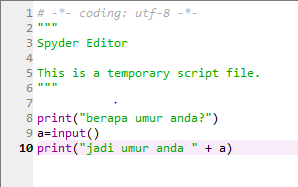
\includegraphics[width=6cm,height=6cm]{figures/c1.png}
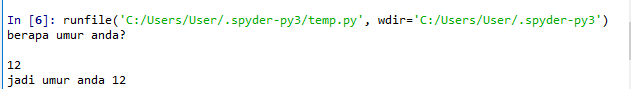
\includegraphics[width=6cm,height=6cm]{figures/c2.png}
\caption {input dan outputnya}
\end{figure}
\begin{figure}
\item asd
\centering
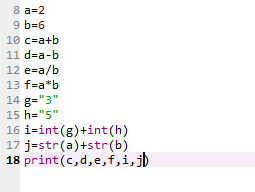
\includegraphics[width=6cm,height=6cm]{figures/c3.png}
\caption{operasi aritmatika}
\end{figure}
\begin{figure}
\item loop digunakan untuk mengulang sampai memenuhi sebuah condition, contoh :
\centering
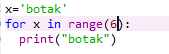
\includegraphics[width=6cm,height=6cm]{figures/c4.png}
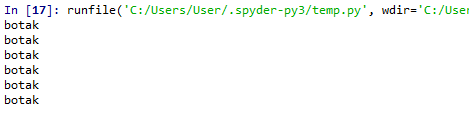
\includegraphics[width=6cm,height=6cm]{figures/c5.png}
\caption {contoh loop/pengulangan}
\end{figure}
\begin{figure}
\item memilih kondisi menggukan syntax if else, cara memakainya yaitu jika sebuah kondisi tidak terpenuhi makan akan meng-execute kondisi lain. contoh:
\centering
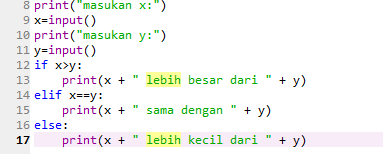
\includegraphics[width=6cm,height=6cm]{figures/c6.png}
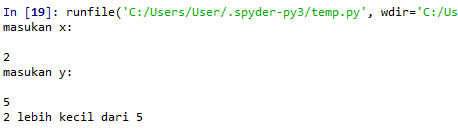
\includegraphics[width=6cm,height=6cm]{figures/c7.png}
\caption{contoh syntax kondisi}
\end{figure}
\begin{figure}
\item asd
\end{figure}
\begin{figure}
\item try berfungsi untuk menguji error, exept berfungsi untuk menangani error. cara memakainya :
\centering
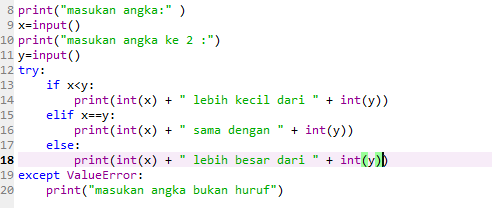
\includegraphics[width=6cm,height=6cm]{figures/c8.png}
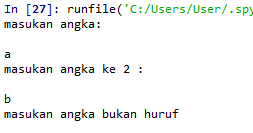
\includegraphics[width=6cm,height=6cm]{figures/c9.png}
\caption{contoh try except}
\end{figure}
\end{enumerate}
\begin{figure}
\subsection{Keterampilan Pemrograman}
\end{figure}
\begin{enumerate}
\begin{figure}
\item a
\end{figure}
\begin{figure}
\item
\center
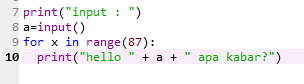
\includegraphics[width=6cm,height=6cm]{figures/c10.png}
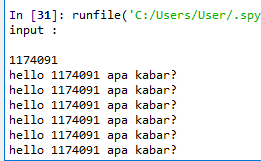
\includegraphics[width=6cm,height=6cm]{figures/c11.png}
\end{figure}
\begin{figure}
\item
\center
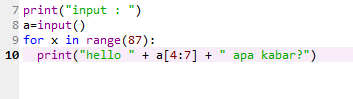
\includegraphics[width=6cm,height=6cm]{figures/c12.png}
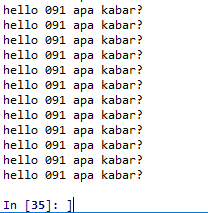
\includegraphics[width=6cm,height=6cm]{figures/c13.png}
\end{figure}
\begin{figure}
\item
\center
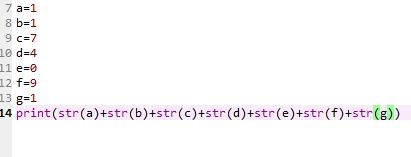
\includegraphics[width=6cm,height=6cm]{figures/c15.png}
\end{figure}
\begin{figure}
\item
\center
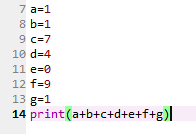
\includegraphics[width=6cm,height=6cm]{figures/c16.png}
\end{figure}
\begin{figure}
\item
\center
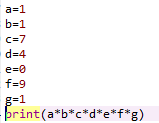
\includegraphics[width=6cm,height=6cm]{figures/c17.png}
\end{figure}
\begin{figure}
\item
\center
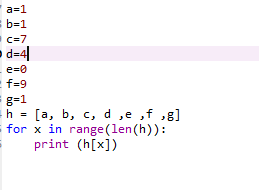
\includegraphics[width=6cm,height=6cm]{figures/c18.png}
\end{figure}
\begin{figure}
\item
\center
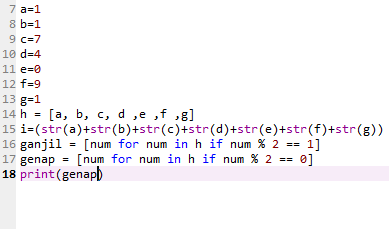
\includegraphics[width=6cm,height=6cm]{figures/c19.png}
\end{figure}
\begin{figure}
\item
\center
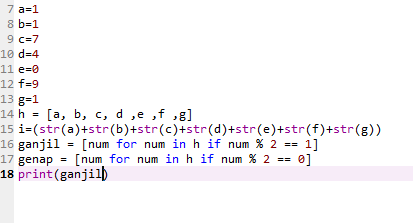
\includegraphics[width=6cm,height=6cm]{figures/c20.png}
\end{figure}
\begin{figure}
\item
\center
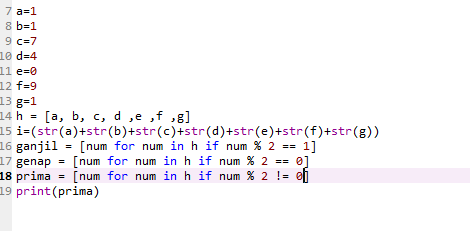
\includegraphics[width=6cm,height=6cm]{figures/c21.png}
\end{figure}
\end{enumerate}




%%%%%%%%%%%%%%%%%%%%%%%%%%%%%%%%%%%%%%%%%%%%%%%%%%%%%%%%%%%%%%%%%%%%%%%%%%%%%%%%%%%%%%%%%
\section{Muhammad Abdul Gani Wijaya}
\subsection{Variable Phyton}
\paragraph{}
Ada beberapa jenis type data pada Phyton, contohnya integer dan string. Penulisan variable seperti berikut :
namavariable = type data, contoh :\\
x = 5\\
y = "John"\\
print(x)\\
print(y)\\
\subsection{Input Phyton}
\paragraph{}
Untuk menampilkan input menggunakan perintah input(). Perintah input() dapat dimasukkan ke dalam variable, sehingga value dari input akan menjadi value dari variable tersebut. Contohnya : \\
print("Enter your name:")\\
x = input()\\
print("Hello, " + x)\\
\subsection{Operator Aritmatika Phyton}
Operator aritmatika dapaat digunakan pada Phyton, seperti + (tambah), - (kurang), * (kali), / (bagi). Contohnya : \\
x9 = 5\\
y9 = 3\\
print(x9 + y9)\\

x10 = 5\\
y10 = 3\\
print(x10 - y10)\\

x11 = 5\\
y11 = 3\\
print(x11 * y11)\\

x12 = 12\\
y12 = 3\\
print(x12 / y12)\\

Untuk mengubah type data menggunakan perintah namavariable = typedata(namavariable yang akan diubah type datatanya). Contoh :\\

x13  = 12\\
y13 = "3"\\
x14 = str(x13)\\
y14 = int(y13)\\
print(x14)\\
print(y14)\\

\subsection{Pengulangan Phyton}
\paragraph{}
Untuk perulangan pada phyton dapat meggunakan perintah while dan for. Contoh :
i = 0\\
while i < 6:\\
  i += 1 \\
  if i == 3:\\
    continue\\
  print(i)\\
  
  fruits = ["apple", "banana", "cherry"]\\
for x in fruits:\\
  print(x)\\
  
 \subsection{Kondisi Phyton}
\paragraph{}
Kondisi juga dapat diterapkan pada phyton, seperti jika a kurang dari b maka b lebih besar dari a. Contohnya :\\
  a = 33\\
b = 200\\
if b > a:\\
  print("b is greater than a")\\
  
 \subsection{Try Except Phyton}
\paragraph{}
Pada phyton seringkali kita menemukan error. Untuk menangkap error dapat menggunakan try except. Contoh :\\

try:\\
  print(x15)\\
except NameError:\\
  print("Variable x15 is not defined")\\
except:\\
  print("Something else went wrong")\\
  
Pada kode tersebut tidak terdapat variable x15 sehingga saat mengeksekusi perintah print(x15) terjadi error. Jika terjadi error karena tida terdapat variable x15 maka outputnya nya menamppilkan "Variable x15 is not defined".

\section{Keterampilan Pemograman}
\subsection{Program}
\lstinputlisting[firstline=8,lastline=62]{src/1174071.py}

\section{Keterampilan Penanganan Error}
\subsection{Program}
\lstinputlisting[firstline=8,lastline=15]{src/Gani2.py}

%%%%%%%%%%%%%%%%%%%%%%%%%%%%%%%%%%%%%%%%%%%%%%%%%%%%%%%%%%%%%%%%%%%%%%
\section{Tia Nur Candida}
\subsection{Jenis Variabel pada Python}
\begin{enumerate}
\item
Bilangan (Number)
Tipe data bilangan umumnya ada 2 yaitu, integer dan float. Integer merupakan bilangan bulat, sedangkan float adalah bilangan pecahan. Terdapat bilangan lain yaitu bilangan kompleks yaitu bilangan yang memiliki bagian real dan imajiner. Integer, float, dan kompleks masing-masing di Python diwakili oleh kelas int, float, dan complex.
\item
String
String merupakan satu atau serangkaian karakter yang diletakkan diantara tanda kutip, baik tanda kutip tunggal ( ‘ ) maupun ganda ( ” ). Huruf, angka, maupun karakter lainnya yang digabung menjadi teks adalah contoh string.
String adalah tipe data yang anggotanya berurut dan memiliki indeks. Indeks dimulai dari angka 0 bila dimulai dari depan dan -1 bila diindeks dari belakang. Tiap karakter bisa diakses menggunakan indeksnya dengan format nama string[indeks] . Pada string juga bisa dilakukan slicing atau mengakses sekelompok substring dengan format namastring[awal:akhir].
\item
List
List merupakan tipe data yang berisi item yang berurut. Seperti halnya tipe data string, tiap item (anggota) list memiliki indeks sesuai dengan urutannya. Indeks dimulai dari 0 dan bukan dari 1.
List bisa berisi anggota dengan tipe yang sama maupun berbeda. Untuk mendeklarasikan list, digunakan tanda kurung [ ] dan masing-masing anggotanya dipisahkan oleh tanda koma.
\item
Tuple
Tuple merupakan jenis data lain yang mirip dengan list. Perbedaannya dengan list adalah anggotanya tidak dapat diubah (immutable). List bersifat mutable, sedangkan tuple bersifat immutable. Sekali tuple dibuat, maka isinya tidak bisa dimodifikasi lagi.
Tuple dideklarasikan dengan menggunakan tanda kurung ( ). dan anggotanya dipisahkan oleh tanda koma. Tuple berguna untuk data yang dimaksudkan tidak diubah isinya. Misalnya tuple komposisi warna untuk putih adalah (255,255,255).
\item
Set
Set merupakan salah satu tipe data pada Python yang tidak berurut (unordered). Set memiliki anggota yang unik (tidak ada duplikasi). Jadi misalnya kalau kita meletakkan dua anggota yang sama di dalam set, maka otomatis set akan menghilangkan yang salah satunya.
Set bisa digunakan untuk melakukan operasi himpunan matematika seperti gabungan, irisan, selisih, dan komplemen.
Set dibuat dengan meletakkan anggota – anggotanya di dalam tanda kurung kurawal { }, dipisahkan menggunakan tanda koma. Kita juga bisa membuat set dari list dengan memasukkan list ke dalam fungsi set()
Set bisa berisi data campuran, baik integer, float, string, dan lain sebagainya. Akan tetapi set tidak bisa berisi list, set, dan dictionary.
\item
Dictionary
Dictionary merupakan tipe data yang tiap anggotanya terdiri dari pasangan kunci-nilai (key-value). Mirip dengan kamus dimana ada kata ada arti. Dictionary umumnya dipakai untuk data yang besar dan untuk mengakses anggota data secara acak. Anggota dictionary tidak memiliki indeks.
Dictionary dideklarasikan dengan menggunakan tanda kurung kurawal { }, dimana anggotanya memiliki bentuk kunci:nilai atau key:value dan tiap anggota dipisah tanda koma. Kunci dan nilainya bisa memiliki tipe sembarang.
\end{enumerate}
\subsection{Cara Menampilkan Output ke Layar}
	Untuk menampilkan Python sudah menyediakan fungsi input() dan rawinput() untuk mengambil inputan dari keyboard.
Cara pakainya: 
Nama variable = input (“Sebuah teks”)
Artinya, teks yang kita inputkan dari keyboard akan disimpan ke dalam nama variabel.
Untuk menampilkan output teks, kita menggunakan fungsi print().
\subsection{Operator Dasar Aritmatika}
\begin{enumerate}
\item
Penjumlahan	+
\item
Pengurangan	-
\item
Perkalian	*
\item
Pembagian	/
\item
Sisa Bagi	(persen)
\item
Pemangkatan	**
\end{enumerate}
\subsection{Jenis dan Sintax Perulangan}
\begin{enumerate}
\item
While Loop\\
While loop dapat mengeksekusi statement selama kondisi nya true
Contoh:
i = 1   \\
while i < 6: \\
  print(i)\\
  i += 1
\item
For Loop\\
For loop digunakan untuk mengulangi urutan (list, tupel, dictionary, set, atau string). Menggunakan for loop dapat mengeksekusi seperangkat statement, satu kali untuk setiap item dalam list, tuple, set dll.\\
Contoh :
fruits = ["apple", "banana", "cherry"]\\
for x in fruits:\\
  print(x)\\

\end{enumerate}
\subsection{Cara Memakai Sintax untuk Memilih Kondisi}
\subsubsection{Kondisi If Else}
	Pengambilan keputusan (kondisi if else) tidak hanya digunakan untuk menentukan tindakan apa yang akan diambil sesuai dengan kondisi, tetapi juga digunakan untuk menentukan tindakan apa yang akan diambil/dijalankan jika kondisi tidak sesuai.
Pada python ada beberapa statement/kondisi diantaranya adalah if, else dan elif Kondisi if digunakan untuk mengeksekusi kode jika kondisi bernilai benar.
Kondisi if else adalah kondisi dimana jika pernyataan benar true maka kode dalam if akan dieksekusi, tetapi jika bernilai salah false maka akan mengeksekusi kode di dalam else.
Dibawah ini adalah contoh penggunaan kondisi if else pada Python\\
Kondisi if else adalah jika kondisi bernilai TRUE maka akan dieksekusi pada if, tetapi jika bernilai FALSE maka akan dieksekusi kode pada else

nilai = 3\\

Jika pernyataan pada if bernilai TRUE maka if akan dieksekusi, tetapi jika FALSE kode pada else yang akan dieksekusi.\\
if(nilai > 7):\\
    print("Selamat Anda Lulus")\\
else:\\
    print("Maaf Anda Tidak Lulus")

\subsection{Jenis Error yang sering ditemui}
\begin{enumerate}
\item
Syntax Errors
Syntax Errors merupakan suatu keadaan saat kode python mengalami kesalahan penulisan. Python interpreter dapat mendeteksi kesalahan ini saat kode dieksekusi.\\
1>>> print"Hello World"\\
2	SyntaxError: invalid syntax\\

Output dari program yang dieksekusi akan menampilkan pesan “invalid syntax“. Penanganan Syntax Errors dilakukan dengan memperbaiki penulisan kode yang salah tersebut. 

\item
Exceptions
Exceptions merupaka suatu keadaan saat penulisan syntax sudah benar, namun kesalahan terjadi karena syntax tidak bisa dieksekusi. Banyak hal yang menyebabkan terjadinya Exceptions, mulai dari kesalahan matematika, kesalahan nama function, kesalahan library, dan lain-lain.\\

Berikut beberapa contoh Exceptions:
\begin{enumerate}
\item
ZeroDivisionError
ZeroDivisonError adalah exceptions yang terjadi saat eksekusi program menghasilkan perhitungan matematika pembagian dengan angka nol (0).
\item
NameError
NameError adalah exception yang terjadi saat kode melakukan eksekusi terhadap local name atau global name yang tidak terdefinisi. Misalnya saat menjumlahkan variable yang tidak didefinisikan, memanggil function yang tidak ada, dan lain-lain.
\item
TypeError
TypeError adalah exception yang terjadi saat dilakukan eksekusi terhadap suatu operasi atau fungsi dengan type object yang tidak sesuai.


\end{enumerate}

\end{enumerate}
\subsection{TryExcept}
Pada kode ini akan mencoba menangkap dua error pada kode yang dikurung oleh try..except. Terdapat sebuah dictionary yang berisi key nama, kota, dan umur. Kemudian kita membuka sebuah file yang bernama contact.txt. Walaupun ada kode error setelahnya yang akan mengakibatkan error pengaksesan indeks, yang akan ditangkap terlebih dahulu adalah error yang diakibatkan gagalnya membaca file.\\
orang = {"nama":"tia", "kota":"sumedang", "umur":"20"}\\

try:\\
    contact = open("contact.txt", 'r')\\
    print orang["pekerjaan"]\\
except IOError, e:\\
    print "Terjadi error IO: ", e\\
except KeyError, e:\\
    print "Terjadi kesalahan pada akses list/dict/tuple:", e\\

print orang


%%%%%%%%%%%%%%%%%%%%%%%%%%%%%%%%%%%%%%%%%%%%%%%%%%%%%%%%%%%%%%%%%%%%%%%%%
\section{Nurul Izza Hamka}
\subsection{Jenis-Jenis Variabel dan Pemakaian Variable di Kode Pyhton :} 
\subsection{Tipe String}
Dalam Python, string direpresentasikan oleh tipe ‘str’. Tipe data string dituliskan di antara dua tanda petik tunggal atau ganda atau kutip ganda tiga kali. \\

Contoh Pemakaian String pada python : \\
x = "Assalamualaikum"\\
print(x)
\\

	Contoh lain Pada pemjumlahan yaitu :
\\
a = "Selamat "\\
b = "Datang"\\
c = a+b\\
print (c)\\

\subsection{Tipe List}
Terdapat dua macam objek list dalam Python, yaitu tuple dan list. Perbedaannya adalah, pada tuple daftar yang dituliskan bersifat tetap dan tidak dapat diubah, sedangkan pada list kita dapat menambah dan menghapus daftar; melakukan penyusunan; dan beberapa jenis modifikasi lainnya. Pemrosesan pada tuple umumnya lebih cepat dibandingkan pemrosesan list, namun karena kemudahan pada proses modifikasi, aturan praktis yang umumnya dianut oleh para programmer Python adalah selalu gunakan list.\\

Contoh :\\
Benda = ["Buku", "Pulpen", "Meja", "Sisir"]\\
print benda [2]

\subsection{Tipe Tuple}
Tuple pada dasarnya mirip dengan list, namun bersifat tetap, tuple mirip dengan array konstan Ketika kita sudah membuatnya, kita tidak dapat melakukan perubahan pada elemen – elemen di dalamnya. Tuple ditulis dengan menggunakan notasi “()”.\\
Contoh : \\
tup1 = ('Aljabar', 'Logistik', 1993, 2017)\\
tup2 = (1, 2, 3, 4, 5 )\\
tup3 = "a", "b", "c", "d"\\
\subsubsection{Tipe Dictionary}

Dictionary adalah salah satu tipe kumpulan objek yang mirip dengan list dan tuple. Namun, perbedaannya adalah dictionary memuat objek yang tidak tersusun. Sebagai gantinya, dictionary menghubungkan relasi satu ke satu (pemetaan) antara kunci (key) ke suatu nilai. Dalam bahasa pemrograman lainnya dikenal sebagai array asosiatif yang indeksnya berupa nama tertentu.\\

Contoh :\\
d = {"Nama" : "Nurul Izza Hamka", "Prodi" : "D IVTeknik Informatika", ... "NPM" : "1174062"}

\section{Kode Untuk Meminta Input Dari User dan Bagaimana Melakukan Output Ke Layar Pada Python ?}
Meminta input atau masukan dari user, prompt sebagai string yang kita ingin tampilkan di layer.  Sintaksnya adalah seperti berikut:\\

input([prompt])\\

Gunakan fungsi print() untuk menampilkan data ke perangkat keluaran standar (layar).\\

 panjang = input('Masukkan nilai panjang: ')\\
Masukkan nilai panjang: 10\\
 lebar = input('Masukkan nilai lebar: ')\\
Masukkan nilai lebar: 5\\
 luas = int(panjang) * int(lebar)\\
 print("Luas =", luas)\\
Luas = 50\\
\section{Operator Dasar Aritmatika, Tambah, Kali, Kurang Bagi dan Bagaimana Mengubah String Ke Integer dan Integer Ke String ?}
Macam-Macam Opertaor Aritmatika :
\subsubsection{Operator Penjumlahan}
Tambah adalah variabel yang digunakan untuk menyimpan hasil penjumlahan. Contoh : variabel a ditambah variabel b ( a + b ).
\subsubsection{Operator Perkalian}
Kali adalah variabel yang digunakan untuk menyimpan hasil perkalian variabel a dikali variabel b ( a *b ).
\subsubsection{Operator Pengurangan}
Kurang adalah variabel yang digunakan untuk menyimpan hasil pengurangan. Contoh : variabel a dikurangvariabel b ( a - b ).
\subsubsection{Operator Pembagian}
Bagi adalah variabel yang digunakan untuk menyimpan hasil pembagian. Contoh : variabel a dibagi variabel b ( a / b ). \\

Cara mengubah Integer ke String :\\
integer ini merupakan tipe data bilangan bulat. Namun kita bisa mengkonversinya ke tipe data string:\\
a=100\\
konversi integer ke string : \\
string = str(a) \\

Cara mengubah String ke Integer :\\
Tipe data string ini merupakan tipe data yang menampung sebuah teks. Namun, kita juga bisa mengkonversi nya ke tipe integer :\\
a ='1212'\\
konversi string ke integer\\
integer = int(a) \\
\section{Sintak Perulangan , Jenis-Jenisnya Contoh dan Cara Pakainya Di Python.}
Terdapat dua jenis perualangan dalam bahasa pemrograman python, yaitu perulangan dengan for dan while. Perulangan for disebut counted loop (perulangan yang terhitung), sementara perulangan while disebut uncounted loop (perulangan yang tak terhitung). Perbedaannya adalah perulangan for biasanya digunakan untuk mengulangi kode yang sudah diketahui banyak perulangannya. Sementara while untuk perulangan yang memiliki syarat dan tidak tentu berapa banyak perulangannya.\\
\subsubsection{Perulangan For}
ulang = 5\\
for i in range(ulang):\\
	print "Perulangan ke-"+str(i)
\subsubsection{Perulangan While}

jawab = 'ya'\\
hitung = 0\\

while(jawab == 'ya'):\\
    hitung += 1\\
    jawab = rawinput("Ulang lagi tidak? ")\\    
print "Total perulagan: " + str(hitung)
\section{Cara Pakai Sintak Untuk Memilih Kondisi dan Bagaimana Contoh Sintak Kondisi Di Dalam Kondisi}
struktuf if dalam Python dijalankan untuk memeriksa apakah kondisi ini adalah bernilai benar atau salah. Jika kondisi ini bernilai true, maka python akan menjalankan statemen didalam blok kondisi tersebut dan sebaliknya jika kondisi bernilai false maka statemen didalam blok tersebut tidak akan dijalankan. 
\subsubsection{If}
x = 1\\
if x lebih dari 0:\\
	print("Nilai persenx adalah besar dari 0" persen x )
\subsubsection{If-else}
If-else\\
umur = 37\\
if umur lebih dari 18 and umur kurang dari 30:\\
    print "Sudah beranjak dewasa"\\
elif umur lebih dari 30 and umur kurang dari 45:\\
    print "Masa - masa emas"\\
elif umur lebih dari 45 and umur kurang dari 55:\\
    print "Memasuki masa paruh baya"\\
elif umur lebih dari 55:\\
    print "Masa - masa manula"\\
else:\\
    print "Masih dibawah umur"
    
\section{Jenis Error  Yang Sering Di Temui Di Python Dalam Mengerjakan Sintak Diatas , dan Bagaimana Cara Mengatasinya ?}

Terdapat 2 jenis error pada Bahasa pemrograman Python yaitu Errors dan Exceptions.
\subsubsection{Syntax Errors}
Syntax Errors adalah suatu keadaan saat kode python mengalami kesalahan penulisan. Python interpreter dapat mendeteksi kesalahan ini saat kode dieksekusi.\\
Output dari program yang dieksekusi akan menampilkan pesan “invalid syntax“. Penanganan Syntax Errors dilakukan dengan memperbaiki penulisan kode yang salah tersebut.
\subsubsection{ Exceptions}
Exceptions adalah suatu keadaan saat penulisan syntax sudah benar, namun kesalahan terjadi karena syntax tidak bisa dieksekusi. Banyak hal yang menyebabkan terjadinya Exceptions, mulai dari kesalahan matematika, kesalahan nama function, kesalahan library, dan lain-lain.\\

Berikut beberapa contoh Exceptions:\\
1. NameError, adalah exception yang terjadi saat kode melakukan eksekusi terhadap local name atau global name yang tidak terdefinisi. Misalnya saat menjumlahkan variable yang tidak didefinisikan, memanggil function yang tidak ada, dan lain-lain.\\
2.TypeError, adalah exception yang terjadi saat dilakukan eksekusi terhadap suatu operasi atau fungsi dengan type object yang tidak sesuai.\\
3. ZeroDivisonError, adalah exceptions yang terjadi saat eksekusi program menghasilkan perhitungan matematika pembagian dengan angka nol (0).\\

Cara penanganan Exceptions yaitu, memasukkan kode yang kamu anggap bisa menimbulkan exception di dalam klausa try. Langkah selanjutnya adalah menggunakan keyword except untuk menangani
exception yang terjadi pada kode berikutnya.\\

Selain itu juga untuk menangani banyak exception menggunakan satu klausa except dengan melewatkan exception tersebut ke klausa sebagai sebuah tuple.

\section{Cara Memakai Try Except}

Blok try memungkinkan Anda menguji blok kode untuk kesalahan.\\
Blok except memungkinkan Anda menangani kesalahan.\\

Jika kesalahan terjadi, eksekusi kode blok try dihentikan dan ditransfer sampai ke blok except. \\
Selain menggunakan blok except setelah blok try, Anda juga dapat menggunakan blok Finally. \\
Kode di blok finally akan dieksekusi terlepas dari apakah except terjadi.\\

\part{Keterampilan Pemrograman}
\begin{enumerate}
	\item No 1
	\lstinputlisting[firstline=7,lastline=18]{src/1174062.py}
	
	\item No 2
	\lstinputlisting[firstline=19,lastline=25]{src/1174062.py}
	
	\item No 3
	\lstinputlisting[firstline=26,lastline=32]{src/1174062.py}
	
	\item No 4
	\lstinputlisting[firstline=33,lastline=36]{src/1174062.py}
	
	\item No 5
	\lstinputlisting[firstline=37,lastline=49]{src/1174062.py}
	
	\item No 6
	\lstinputlisting[firstline=50,lastline=52]{src/1174062.py}
	
	\item No 7
	\lstinputlisting[firstline=53,lastline=56]{src/1174062.py}
	
	\item No 8
	\lstinputlisting[firstline=57,lastline=65]{src/1174062.py}
	
	\item No 9
	\lstinputlisting[firstline=66,lastline=68]{src/1174062.py}
	
	\item No 10
	\lstinputlisting[firstline=69,lastline=71]{src/1174062.py}
	
\end{enumerate}


\part{Ketrampilan Penanganan Error}


%%%%%%%%%%%%%%%%%%%%%%%%%%%%%%%%%%%%%%%%%%%%%%%%%%%%%%%%%%%%%%%%%%%%%%%%%%%%
\section{Aulyardha Anindita}
\section{Jenis-jenis Variabel}
\subsection{Bilangan (Number)}
Pada bilangan (Number) ada dua yang sering dipakai, yaitu : integer dan float.Integer adalah bilangan bulat, sedangkan float adalah bilangan pecahan. Selain itu ada tipe bilangan lain, yaitu bilangan kompleks yaitu bilangan yang memiliki bagian real dan imajiner. Integer, float, dan kompleks masing-masing di Python diwakili oleh kelas int, float, dan complex.\\
Contoh kode phyton :\\
x = 5 \\
print(x, "angkanya adalah ", type(x))\\
x = 2.5\\
print(x, "angkanya adalah ", type(x))\\

\subsection{String}
String adalah satu atau serangkaian karakter yang diletakkan diantara tanda kutip, baik tanda kutip tunggal ( ‘ ) maupun ganda ( ” ). Huruf, angka, maupun karakter lainnya yang digabung menjadi teks adalah contoh string. String adalah tipe data yang anggotanya berurut dan memiliki indeks. Indeks dimulai dari angka 0 bila dimulai dari depan dan -1 bila diindeks dari belakang. Tiap karakter bisa diakses menggunakan indeksnya dengan formatnamastring[indeks] . Pada string juga bisa dilakukan slicing atau mengakses sekelompok substring dengan format namastring[awal:akhir] \\
Contoh kode phyton :\\
kalimat = "Nama saya Aulyardha Anindita"\\
print(kalimat)\\
print(kalimat[0])\\
print(kalimat[-1])\\
print(kalimat[4:7])\\
print(kalimat[:4])\\

\subsection{List}
List adalah tipe data yang berisi item yang berurut. Seperti halnya tipe data string, tiap item (anggota) list memiliki indeks sesuai dengan urutannya. Indeks dimulai dari 0 dan bukan dari 1. List bisa berisi anggota dengan tipe yang sama maupun berbeda. Untuk mendeklarasikan list, digunakan tanda kurung [ ] dan masing-masing anggotanya dipisahkan oleh tanda koma.\\
Contoh kode phyton :\\
a = [5,10,15,20,25,30,35,40]\\
a[2] = 15\\
print("a[2] = ", a[2])\\
a[0:3] = [5, 10, 15]\\
print("a[0:3] = ", a[0:3])\\
a[5:] = [30, 35, 40]\\
print("a[5:] = ", a[5:])\\

\subsection{Tuple}
Tuple adalah jenis data lain yang mirip dengan list. Perbedaannya dengan list adalah anggotanya tidak bisa diubah (immutable). List bersifat mutable, sedangkan tuple bersifat immutable. Sekali tuple dibuat, maka isinya tidak bisa dimodifikasi lagi. Tuple dideklarasikan dengan menggunakan tanda kurung ( ). dan anggotanya dipisahkan oleh tanda koma. Tuple berguna untuk data yang dimaksudkan tidak diubah isinya. Misalnya tuple komposisi warna untuk putih adalah\\ (255,255,255).
Contoh kode phyton :\\
white = (255,255, 255)\\
red = (255,0,0)\\
print(white)\\
print(red[0])\\
print(red[1])\\
red[0] = 128\\

\subsection{Set}
Set adalah salah satu tipe data di Python yang tidak berurut (unordered). Set memiliki anggota yang unik (tidak ada duplikasi). Jadi misalnya kalau kita meletakkan dua anggota yang sama di dalam set, maka otomatis set akan menghilangkan yang salah satunya. Set bisa digunakan untuk melakukan operasi himpunan matematika seperti gabungan, irisan, selisih, dan komplemen. Set dibuat dengan meletakkan anggota – anggotanya di dalam tanda kurung kurawal { }, dipisahkan menggunakan tanda koma. Kita juga bisa membuat set dari list dengan memasukkan list ke dalam fungsi set() Set bisa berisi data campuran, baik integer, float, string, dan lain sebagainya. Akan tetapi set tidak bisa berisi list, set, dan dictionary.\\
Contoh Kode Phyton : \\
myset = {1,2,3} \\
print(myset) \\

\subsection{Dictionary}
Dictionary adalah tipe data yang tiap anggotanya terdiri dari pasangan kunci-nilai (key-value). Mirip dengan kamus dimana ada kata ada arti. Dictionary umumnya dipakai untuk data yang besar dan untuk mengakses anggota data secara acak. Anggota dictionary tidak memiliki indeks. Dictionary dideklarasikan dengan menggunakan tanda kurung kurawal { }, dimana anggotanya memiliki bentuk kunci:nilai atau key:value dan tiap anggota dipisah tanda koma. Kunci dan nilainya bisa memiliki tipe sembarang.\\
Contoh Kode Phyton : \\
d = {1:'satu', 2:'dua', 'tiga':3}\\
print(tipe(d))\\
print("d[1] = ", d[1])\\
print("d['tiga'] = ", d['tiga'])\\

\section{Cara Meminta Input Kepada User dan Bagaimana Outputnya}
Input adalah masukan yang kita berikan ke program.
Program akan memprosesnya dan menampilkan hasil outputnya.Input, proses, dan output adalah inti dari semua program komputer.\\
\subsection{Input}
Python sudah menyediakan fungsi input() dan rawinput() untuk mengambil inputan dari keyboard.\\
Contoh :\\
nama = rawinput("Nama Kamu Siapa?: ")\\
umur = input("Umur Kamu Berapa: ")\\

Akan menampilkan output :\\
print "Hello",nama,"umur kamu adalah",umur,"tahun"\\
"Hello Dita, umur kamu adalah 19 Tahun"\\
\subsection{Output}
Untuk menampilkan output teks, kita menggunakan fungsi print().\\
Contoh :\\
nama = "Aulyardha Anindita"\\
print "Hello",nama\\
Hasil :\\
"Hello Aulyardha Anindita"\\

\section{Operator Dasar Aritmetika dan Cara Mengubah String ke Int Begitu Juga Sebaliknya}
\subsection{Operator Dasar Aritmetika}
\begin{enumerate}
\item + = Penjumlahan, Contoh : x+y\\
\item - = Pengurangan, Contoh : x-y\\
\item * = Perkalian, Contoh : x*y\\
\item / = Pembagian, Contoh : x/y\\
\item Persen = Modulus, Contoh:	x persen y\\
\item ** = Exponentiation, Contoh :	x ** y\\
\item // = Floor division, Contoh :	x // y\\
\end{enumerate}
\subsection{Cara Mengubah String Ke Int Sebaliknya}
\subsubsection{String ke Int}
Tipe data string merupakan tipe data yang menampung sebuah teks. tipe data string juga bisa dikonversi ke int. Tidak boleh ada satu karakter pun yang berupa huruf. Jika ada hurufnya, maka kita akan mendapatkan error. \\
Contoh Kode :\\
a ='1234' \\
integer = int(a)\\
print(integer)\\

\subsubsection{Int ke String}
Tipe data integer ini merupakan tipe data bilangan bulat. Namun kita bisa mengkonversinya ke tipe data yang lain. Seperti string, float, complex, dan long.\\ Contoh Kode :\\
a=40\\
string = str(a)\\
print(string)\\

\section{Perulangan}
\subsection{While loop}
Dengan while loop , kita dapat menjalankan serangkaian pernyataan selama suatu kondisi benar.\\
Contoh Kode :\\
i = 1\\
while i < 6:\\
  print(i)\\
  if i == 3:\\
    break\\
  i += 1\\
\subsection{For Loop}
For loop digunakan untuk mengulangi urutan (baik dalam bentuk list, tuple, dictionary, set atau string.
Dengan for loop kita dapat mengeksekusi seperangkat pernyataan, satu kali untuk setiap item dalam daftar, tuple, set dll.\\
Contoh Kode :\\
hewan = ["Kelinci", "Serangga", "Kupu-kupu"]\\
for x in hewan:\\
  if x == "Kelinci":\\
    break\\
  print(x)\\

\section{Kondisi}
\subsection{If}
If digunakan untuk mengantisipasi kondisi yang terjadi saat jalanya program dan menentukan tindakan apa yang akan diambil sesuai dengan kondisi. Jika kondisi bernilai salah False maka statement/kondisi if tidak akan di-eksekusi.\\
Contoh Kode :\\
nilai = 8\\
if(nilai > 7):\\
    print("Selamat Anda Lulus")\\
if(nilai > 10):\\
    print("Selamat Anda Lulus")\\

\subsection{If else}
Pengambilan keputusan (kondisi if else) tidak hanya digunakan untuk menentukan tindakan apa yang akan diambil sesuai dengan kondisi, tetapi juga digunakan untuk menentukan tindakan apa yang akan diambil/dijalankan jika kondisi tidak sesuai.

Kondisi if else adalah kondisi dimana jika pernyataan benar True maka kode dalam if akan dieksekusi, tetapi jika bernilai salah False maka akan mengeksekusi kode di dalam else.\\
Contoh :\\
nilai = 3\\
if(nilai > 7):\\
    print("Selamat Anda Lulus")\\
else:\\
    print("Maaf Anda Tidak Lulus")\\
    
\subsection{Elif}
Pengambilan keputusan (kondisi if elif) merupakan lanjutan/percabangan logika dari “kondisi if”. Dengan elif kita bisa membuat kode program yang akan menyeleksi beberapa kemungkinan yang bisa terjadi. Hampir sama dengan kondisi “else”, bedanya kondisi “elif” bisa banyak dan tidak hanya satu.\\
Contoh Kode :\\
hariini = "Minggu"\\
if(hariini == "Senin"):\\
    print("Saya akan kuliah")\\
elif(hariini == "Selasa"):\\
    print("Saya akan kuliah")\\
elif(hariini == "Rabu"):\\
    print("Saya akan kuliah")\\
elif(hariini == "Kamis"):\\
    print("Saya akan kuliah")\\
elif(hariini == "Jumat"):\\
    print("Saya akan kuliah")\\
elif(hariini == "Sabtu"):\\
    print("Saya akan kuliah")\\
elif(hariini == "Minggu"):\\
    print("Saya akan libur")\\
    
\section{Jenis Error}
\subsection{Syntax errors}
Python hanya dapat mengeksekusi sebuah program hanya jika program tersebut
berisi baris - baris perintah dengan sintaks yang benar. Kalau dalam program tersebut terdapat kesalahan sintaks maka proses akan berhenti dan menampilkan 
pesan kesalahan, yang kemudian dikenal sebagai Syntax errors . Sintaks merujuk ke sebuah struktur program dan aturan - aturan yang berperan dalam struktur 
tersebut, kalimat tersebut akan mempunyai kesalahan sintaks jika penulisan kalimat tidak sesuai dengan aturan yang berlaku. 
\subsection{Runtime errors}
Jenis kesalahan kali ini disebut dengan runtime errors, disebut begitu karena kesalahan tidak akan muncul sampai Anda menjalankan program tersebut. Kesalahan ini juga dikenal dengan exceptions atau pengecualian karena biasanya mengindikasikan sesuatu pengecualian yang buruk telah terjadi. Runtime errors sangat jarang terjadi pada program sederhana pada contoh 
beberapa bab pertama.
\subsection{Semantic errors}
Jika terdapat kesalahan jenis ini dalam program Anda, program masih akan berjalan dengan lancar dan tidak mengeluarkan pesan kesalahan, tetapi tidak
akan sesuai dengan harapan, karna akan terjadi penyimpangan dan berbeda dengan 
apa yang diinginan. Karena program tersebut tidak sesuai dengan yang diharapkan dan akan meminta
Anda untuk menelusuri kembali program tersebut dari awal untuk memperbaiki
algoritmanya, kesalahan ini akan sering muncul pada saat Anda mulai berpengalaman dengan suatu bahasa pemograman.
\subsection{Debugging}
Debugging merupakan kekayaan intelektual seseorang yang paling tinggi,menantang dan bagian yang paling menarik dari pemograman. Menurut pendapat beberapa orang, pemograman dan debugging adalah hal yang
sama. Jadi pemograman adalah sebuah proses yang harus melalui proses beberapa kali debugging untuk mendapatkan hasil yang Anda inginkan. Dalam proses debugging, suatu komentar instruksi program sangat berguna sekali dalam pembacaan suatu kode. Pada umumnya komentar berisi keterangan tentang
kegunaan suatu fungsi itu. Sintaksnya adalah tanda kres atau tanda pagar. Setelah meletakkan tanda tersebut, kita dapat mengetikan kalimat apa saja yang
berhubungan dengan suatu instruksi perintah, sebab apapun kalimat tersebut tidak
akan di proses oleh interpreter. 
\subsection{Exceptions}
Jika terjadi kesalahan pada saat program dijalankan (run-time errors), program tersebut membuat sebuah pengecualian (exceptions). Biasanya program terhenti
dan menampilkan pesan kesalahan.Pada setiap kasus, pesan kesalahan dibagi menjadi dua bagian: Jenis kesalahan sebelum titik dua, dan menjelaskan secara spesifik tentang kesalahan tersebut
dibagian setelah titik dua. Pada umumnya, interpreter Python juga menampilkan sebuah penulusuran kembali dimana kesalahan pada program tersebut, yang dapat
kita lihat sebelumnya.

\section{Cara Memakai Try Except}
Kode di awal artikel meminta pengguna untuk memasukkan integer sebagai sebuah input. Jika penggunanya tidak menyediakan masukkan integer, program-nya akan menghentikan eksekusi dan memunculkan nilai error exception-nya. Pada bagian ini, kita akan menulis beberapa kode untuk memberi tahu pengguna bahwa masukkan mereka bukanlah nilai integer yang valid.

Langkah pertama dari prosesnya adalah memasukkan kode yang kamu anggap bisa menimbulkan exception di dalam klausa try. Langkah selanjutnya adalah menggunakan keyword except untuk menangani exception yang terjadi pada kode di atas. Kode yang dimodifikasi untuk masukkan penggunanya akan tampak seperti berikut:\\\\
1\\
2\\
3\\
4\\
5\\
6\\
7\\
8\\
keepasking = True\\ 
while keepasking:\\
    try:\\
        x = int(input("Please enter a number: "))\\
        print("Dividing 50 by", x,"will give you :",50/x)\\
    except ValueError:\\
        print("The input was not an integer. Please try again...")\\\\
Apa yang terjadi di sini adalah program-nya mencoba untuk mengeksekusi kodenya di dalam klausa try. Jika tidak ada exception yang muncul, programnya akan melewati klause except dan sisa kode-nya akan dieksekusi secara normal. Jika sebuah exception muncul, program-nya akan melewatkan sisa kode di dalam klausa try dan tipe dari exception-nya akan dicocokkan dengan nama exception setelah keyword except. Dalam kasus yang cocok, kode di dalam klausa except akan dieksekusi terlebih dahulu dan sisa setelah klausa try akan dieksekusi secara normal.

Ketika kamu memasukkan sebuah integer sebagai masukkannya, program-nya memberikanmu hasil akhir dari pembagian. Ketika nilai non-integral disediakan, program-nya akan mencetak sebuah pesan memintamu untuk mencoba dan memasukkan sebuah integer lagi. Ingat kali ini, programnya tidak akan keluar secara paksa saat kamu memasukkan nilai yang tidak valid.

Kamu bisa memiliki banyak klausa except untuk menangai aneka exceptions. Tolong diingat bahwa handler hanya akan menangani exception yang terjadi dan berkoreponsi dengan klausa try. Mereka tidak akan menangani exception apapun yang muncul di handler exception yang lainnya.

\part{Keterampilan Pemrograman}
\begin{enumerate}
	\item Jawaban soal no 1
    \lstinputlisting[firstline=9, lastline=20]{src/1174054.py}
    \item Jawaban soal no 2
    \lstinputlisting[firstline=21, lastline=27]{src/1174054.py}
    \item Jawaban soal no 3
    \lstinputlisting[firstline=28, lastline=34]{src/1174054.py}
    \item Jawaban soal no 4
    \lstinputlisting[firstline=35, lastline=38]{src/1174054.py}
    \item Jawaban soal no 5
    \lstinputlisting[firstline=39, lastline=51]{src/1174054.py}
    \item Jawaban soal no 6
    \lstinputlisting[firstline=52, lastline=54]{src/1174054.py}
    \item Jawaban soal no 7
    \lstinputlisting[firstline=55, lastline=57]{src/1174054.py}
    \item Jawaban soal no 8
    \lstinputlisting[firstline=58, lastline=66]{src/1174054.py}
    \item Jawaban soal no 9
    \lstinputlisting[firstline=67, lastline=69]{src/1174054.py}
    \item Jawaban soal no 10
    \lstinputlisting[firstline=70, lastline=72]{src/1174054.py}
    \item Jawaban soal no 11
    \lstinputlisting[firstline=73, lastline=75]{src/1174054.py}
\end{enumerate}

\part{Keterampilan Penanganan Error}
\lstinputlisting[firstline=8, lastline=17]{src/2err_1174054.py}

%%%%%%%%%%%%%%%%%%%%%%%%%%%%%%%%%%%%%%%%%%%%%%%%%%%%%%%%%%%%%%%%%%%%%%%%%%%%%%%%%%%%%%%%%%%%%%%%%%%%%
\section{Difa Al Fansha}
\subsection{Teori}

\begin{enumerate}
\item Variabel merupakan tempat menyimpan data
Aturan Penulisan Variabel :
\begin{itemize}
\item Nama variabel boleh diawali menggunakan huruf atau garis bawah.
\item Karakter selanjutnya dapat berupa huruf, garis bawah atau angka.
\item Karakter pada nama variabel bersifat sensitif (case-sensitif). Artinya huruf besar dan kecil dibedakan. 
\item Nama variabel tidak boleh menggunakan kata kunci yang sudah ada dalam python seperti if, while, for, dsb.
\end{itemize}
'Contoh :'
\begin{verbatim}
x = 21
y = "Difa Al Fansha"
print(x)
print(y)
\end{verbatim}

\item Input adalah masukan yang kita berikan ke program dan program akan memproses dan menampilkan hasil outputnya.\\
'Contoh :'
\begin{verbatim}
# Mengambil input
nama = input("Siapa nama kamu : ")
umur = input("Berapa umur kamu : ")

# Menampilkan output
print ("Hello",nama,"umur kamu adalah",umur,"tahun")
\end{verbatim}

\item Operator Dasar Aritmatika.\\
'Contoh :'
\begin{verbatim}
a = 21
b = 7
c = "Difa Al Fansha"
d = "17"
# Tambah
print (a + b)
# Kurang
print (a - b)
# Kali
print (a * b)
# Bagi
print (a / b)
# String ke int
print ("Nama :",c, "Dan", "Umur :", int(d))
# Int ke String
print (str(a) + str(b))
\end{verbatim}

\item Perulangan\\
'Contoh :'
\begin{verbatim}
# For Loops
Nama = ["Difa Al Fansha"]
for x in Nama :
    print (x)
    
# While Loops
e = 1
while e < 6 :
    print (e)
    e += 1
\end{verbatim}

\item Kondisi if  ini bisa digunakan beberapa cara, kondisi if digunakan jika user memerlukan kondisi yang memerlukan pernyatan.\\
'Contoh :'
\begin{verbatim}
f = 50
g = 200
if g > f :
    print ("G Lebih besar dari F")
    if g == 200:
        print ("Nilai G adalah 200")
\end{verbatim}

\item Error yang sering ditemui\\
SyntaxError: invalid syntax\\
Cara mengatasi\\
\begin{verbatim}
f = 50
g = 200
if g > f :
    print ("G Lebih besar dari F")
    if g == 200:
        print ("Nilai G adalah 200")
else :
    print ("F Lebih besar dari G")
\end{verbatim}

\item Ketika sebuah error ditemukan, untuk mengatasi itu, pernyatan try dan except.\\
Try berfungi untuk menangkap error, dan except berguna untuk mengatasi error tersebut.\\
Apabila try benar, sistem akan menjalan try dan tidak mengekseksi except, apabila try teradpat error , sistem akan menjalankan except.\\
\begin{verbatim}
try :
    print (Hello)
except :
    print ("Ada yang salah")
\end{verbatim}
\end{enumerate}

\section{Ketrampilan Pemrogaman}

\begin{enumerate}
\item Jawaban Nomor 1
\lstinputlisting[firstline=73, lastline=81]{src/1174076.py}

\item Jawaban Nomor 2
\lstinputlisting[firstline=84, lastline=88]{src/1174076.py}

\item Jawaban Nomor 3
\lstinputlisting[firstline=91, lastline=95]{src/1174076.py}

\item Jawaban Nomor 4
\lstinputlisting[firstline=98, lastline=99]{src/1174076.py}

\item Jawaban Nomor 5
\lstinputlisting[firstline=102, lastline=114]{src/1174076.py}

\item Jawaban Nomor 6
\lstinputlisting[firstline=117, lastline=117]{src/1174076.py}

\item Jawaban Nomor 7
\lstinputlisting[firstline=120, lastline=120]{src/1174076.py}

\item Jawaban Nomor 8
\lstinputlisting[firstline=123, lastline=124]{src/1174076.py}

\item Jawaban Nomor 9
\lstinputlisting[firstline=127, lastline=130]{src/1174076.py}

\item Jawaban Nomor 10
\lstinputlisting[firstline=134, lastline=137]{src/1174076.py}

\item Jawaban Nomor 11
\lstinputlisting[firstline=140, lastline=143]{src/1174076.py}
\end{enumerate}

\section{Keterampilan Penanganan Error}
\begin{enumerate}
\item Jawaban Nomor 1  : Error
\begin{verbatim}
a = 100
b = "50"
    c = a + b
    print("Hasil :", c)
\end{verbatim}

\item Jawaban Nomor 2 : Solusi
\begin{verbatim}
a = 100
b = "50"

try:
    c = a + int(b)
    print("Hasil :", c)
except TypeError :
    print("Tipe data tidak sama") 
\end{verbatim}

\end{enumerate}


%%%%%%%%%%%%%%%%%%%%%%%%%%%%%%%%%%%%%%%%%%%%%%%%%%%%%%%%%%%%%%%%%%%%%%%5
\section{Ilham Muhammad Ariq}
\subsection{Teori}
\begin{enumerate}
    \item sebutkan jenis-jenis variabel dan jelaskan cara pemakaian variabel tersebut di
    kode Python
    Variabel merupakan tempat menyimpan data. Kemudian didalam phyton kita dapat membuat variable dengan berbagai cara, yakni sebagai berikut
    \lstinputlisting[firstline=8, lastline=51]{src/1174087.py}

    \item tuliskan bagaimana kode untuk meminta input dari user dan tuliskan bagaimana
    melakukan output ke layar.
    \lstinputlisting[firstline=53, lastline=56]{src/1174087.py}

    \item Tuliskan operator dasar aritmatika, tambah, kali, kurang bagi, dan bagaimana
    mengubah string ke integer dan integer ke string
    Operator  aritmatika adalah operator yang digunakan untuk melakukan suatu perhitungan pada program
    \lstinputlisting[firstline=58, lastline=68]{src/1174087.py}

    \item Tuliskan dan jelaskan sintak untuk perulangan, jenis-jenisnya contoh kode dan
    cara pakainya di python
    Untuk Perulangan Pada Python ada For dan While, contoh ada dibawah ini :
    \lstinputlisting[firstline=70, lastline=80]{src/1174087.py}

    \item Tuliskan jelaskan cara pakai sintak untuk memilih kondisi, dan bagiamana contoh sintak kondisi 		di dalam kondisi.
    Pengambilan kondisi If yang digunakan untuk mengantisipasi kondisi yang terjadi saat program 				dijalankan dan menentukan tindakan apa yang akan diambil sesuai dengan kondisi.
    If statement
    \lstinputlisting[firstline=83, lastline=86]{src/1174087.py}
    
    If Else
    \lstinputlisting[firstline=88, lastline=93]{src/1174087.py}
    
    Elif
    \lstinputlisting[firstline=95, lastline=103]{src/1174087.py}

    \item Tuliskan apa saja jenis error yang sering ditemui di python dalam mengerjakan
    sintak diatas. dan bagaimana cara mengatasinya
    \begin{itemize}
        \item Exception
        Kelas dasar untuk semua pengecualian / exception

        \item Stoplteration
        Dibesarkan ketika metode (iterator) berikutnya dari iterator tidak mengarah ke objek apa pun.

        \item SystemExit
        Dibesarkan oleh fungsi sys.exit ().

        \item StandardError
        Kelas dasar untuk semua pengecualian built-in kecuali StopIteration dan SystemExit.

        \item ArithmeticError
        Kelas dasar untuk semua kesalahan yang terjadi untuk perhitungan numerik.

        \item OverflowError
        Dibesarkan saat perhitungan melebihi batas maksimum untuk tipe numerik.

        \item FloatingPointError
        Dibesarkan saat perhitungan floating point gagal.

        \item ZeroDivisonError
        Dibesarkan saat pembagian atau modulo nol dilakukan untuk semua tipe numerik.

        \item AssertionError
        Dibesarkan jika terjadi kegagalan pernyataan Assert.

        \item AttributeError
        Dibesarkan jika terjadi kegagalan referensi atribut atau penugasan.
         
        \item EOFError
        Dibesarkan bila tidak ada input dari fungsi rawinput () atau input () dan akhir file tercapai.

        \item ImportError
        Dibesarkan saat sebuah pernyataan impor gagal.

        \item KeyboardInterrupt
        Dibesarkan saat pengguna menyela eksekusi program, biasanya dengan menekan Ctrl + c.

        \item LookupError
        Kelas dasar untuk semua kesalahan pencarian.

        \item IndexError
        Dibesarkan saat sebuah indeks tidak ditemukan secara berurutan.

        \item KeyError
        Dibesarkan saat kunci yang ditentukan tidak ditemukan dalam kamus.

        \item NameError
        Dibesarkan saat pengenal tidak ditemukan di namespace lokal atau global.

        \item UnboundLocalError
        Dibesarkan saat mencoba mengakses variabel lokal dalam suatu fungsi atau metode namun tidak ada 			nilai yang ditugaskan padanya.

        \item EnvironmentError
        Kelas dasar untuk semua pengecualian yang terjadi di luar lingkungan Python.

        \item IOError
        Dibesarkan saat operasi input / output gagal, seperti pernyataan cetak atau fungsi open () saat 			mencoba membuka file yang tidak ada.

        \item OSError
        Dibangkitkan untuk kesalahan terkait sistem operasi.

        \item SyntaxError
        Dibesarkan saat ada kesalahan dengan sintaks Python.

        \item IndentationError
        Dibesarkan saat indentasi tidak ditentukan dengan benar.

        \item SystemError
        Dibesarkan saat penafsir menemukan masalah internal, namun bila kesalahan ini ditemui juru bahasa 		Python tidak keluar.

        \item SystemExit
        Dibesarkan saat juru bahasa Python berhenti dengan menggunakan fungsi sys.exit (). Jika tidak 				ditangani dalam kode, menyebabkan penafsir untuk keluar.

        \item TypeError
        Dibesarkan saat operasi atau fungsi dicoba yang tidak valid untuk tipe data yang ditentukan.

        \item ValueError
        Dibesarkan ketika fungsi bawaan untuk tipe data memiliki jenis argumen yang valid, namun argumen 			tersebut memiliki nilai yang tidak valid yang ditentukan.

        \item RuntimeError
        Dibesarkan saat kesalahan yang dihasilkan tidak termasuk dalam kategori apa pun.

        \item NotImplementedError
        Dibesarkan ketika metode abstrak yang perlu diimplementasikan di kelas warisan sebenarnya tidak 			dilaksanakan.
    \end{itemize}

    \item Tuliskan dan jelaskan cara memakai Try Except.
    \lstinputlisting[firstline=105, lastline=111]{src/1174087.py}

\end{enumerate}
\subsection{Ketrampilan Pemrograman}
\begin{enumerate}
    \item Buatlah luaran huruf yang dirangkai dari tanda bintang, pagar atau plus dari NPM kita. Tanda 		    bintang untuk NPM mod 3=0, tanda pagar untuk NPM mod 3 =1, tanda plus untuk NPM mod3=2.
    \lstinputlisting[firstline=114, lastline=121]{src/1174087.py}

    \item  Buatlah program hello word dengan input NPM yang disimpan dalam sebuah variabel string bernama      	NPM dan output sebanyak dua dijit belakang NPM, contoh NPM : 113040087 maka akan ada output sebanyak 		87 dengan tulisan ‘Hallo, 113040087 apa kabar?’
    \lstinputlisting[firstline=123, lastline=128]{src/1174087.py}
    
    \item Buatlah program hello word dengan input nama yang disimpan dalam sebuah
    variabel string bernama NPM dan beri luaran output berupa tiga karakter
    belakang dari NPM sebanyak penjumlahan tiga dijit tersebut.
    \lstinputlisting[firstline=130, lastline=135]{src/1174087.py}

    \item Buatlah program hello word dengan input nama yang disimpan dalam sebuah variabel string bernama 	NPM dan beri luaran output berupa digit ketiga dari belakang dari variabel NPM,
    \lstinputlisting[firstline=137, lastline=139]{src/1174087.py}
    
    \item  (untuk soal no 5 dan selanjutnya) buat program dengan mengisi variabel alfabet dengan nomor 			npm satu persatu berurut. 
    \lstinputlisting[firstline=141, lastline=149]{src/1174087.py}

    \item Dari soal no 5, Lakukan penjumlahan dari seluruh variabel tersebut.
    \lstinputlisting[firstline=151, lastline=152]{src/1174087.py}

    \item Dari soal no 5, Lakukan perkalian dari seluruh variabel tersebut.
    \lstinputlisting[firstline=154, lastline=155]{src/1174087.py}

    \item Dari soal no 5, Lakukan print secara vertikal dari NPM anda menggunakan
    variabel diatas.
    \lstinputlisting[firstline=157, lastline=160]{src/1174087.py}

    \item Dari soal no 5, Lakukan print NPM anda tapi hanya dijit genap saja.
    \lstinputlisting[firstline=162, lastline=166]{src/1174087.py}

    \item Dari soal no 5, Lakukan print NPM anda tapi hanya dijit ganjil saja.
    \lstinputlisting[firstline=168, lastline=171]{src/1174087.py}

    \item Dari soal no 5, Lakukan print NPM anda tapi hanya dijit yang termasuk bilangan prima saja.
    \lstinputlisting[firstline=173, lastline=174]{src/1174087.py}

\end{enumerate}
\subsection{Keterampilan Penanganan Error}
    \lstinputlisting[language=Python]{src/2erry_1174087.py}
	

%%%%%%%%%%%%%%%%%%%%%%%%%%%%%%%%%%%%%%%%%%%%%%%%%%%%%%%%%%%%%%%%%%%%%%%%%%%%%%%%
\section{Muhammad Reza Syachrani / 1174084}
\subsection{Teori}
\begin{enumerate}
\item Variable dibuat saat anda pertama kali memberikan nilai padanya yang merupakan tempat penyimpanan untuk teks dan angka, variable juga tidak perlu dideklarasikan dengan tipe tertentu dan dapat mengubah jenisnya setelah sudah ditetapkan. Variabel selalu ditugaskan dengan tanda sama dengan, diikuti oleh nilai variable dan harus memiliki nama sehingga kita dapat menemukannya lagi. Aturan untuk variabel Python:

\begin{itemize}
    \item Nama variable harus dimulai dengan huruf atau karakter garis bawah
    \item Nama variable tidak dapat dimulai dengan angka
    \item Nama variable hanya dapat berisi karakter alfanumerik dan garis bawah (A-z, 0-9, dan "-")
    \item Nama variable tidak bisa menggunakan kata yang disediakan untuk Python.
\end{itemize}

    \item Kode untuk meminta inputan dari pengguna yaitu menggunakan perintah “ input()  “  dan apabila ingin menampilkan output pada layer menggunakan perintah “ print() ”.
    \item Operator dasar aritmatika :
    \begin{itemize}
    \item Tambah (+)
     \par Contoh : x + y
    \item Kurang (-)
    \par Contoh : x - y
    \item kali (*)
    \par Contoh : x * y
    \item Bagi (/)
    \par Contoh : x / y
    \end{itemize}
\par Cara mengubah tipe data string ke integer :
\lstinputlisting[firstline=8, lastline=9]{src/1174084.py}
\par Cara mengubah tipe data integer ke string :
\lstinputlisting[firstline=11, lastline=12]{src/1174084.py}

\item  Pada perulangan terdapat dua jenis di dalam phyton yaitu perulangan while dan perulangan for
\begin{itemize}
    \item Perulangan while :
    \lstinputlisting[firstline=15, lastline=18]{src/1174084.py}
    \item Perulangan for :
    \lstinputlisting[firstline=20, lastline=22]{src/1174084.py}
\end{itemize}

\item sintak Untuk memilih kondisi, dan kondisi didalam kondisi
\begin{itemize}

\item If
Kondisi ini dipergunakan jika penkondisiannya hanya satu.
\lstinputlisting[ firstline=25, lastline=28]{src/1174084.py}

\item Elif
Kondisi ini dipergunakan jika pengkondisiannya lebih dari dua dan jika kondisi sebelumnya tidak benar, maka coba kondisi ini akan dijalankan
\lstinputlisting[ firstline=30, lastline=35]{src/1174084.py}

\item Kondisi di dalam kondisi
Kondisi ini dipergunakan jika pengkondisiannya memerlukan pengkondisian di dalamnya.
\lstinputlisting[ firstline=38, lastline=48]{src/1174084.py}
\end{itemize}
 
\item Jenis-jenis error yang terjadi dan cara mengatasinya pada Python
\begin{itemize}
    \item Type Error
    \par TypeError merupakan exception yang terjadi saat dilakukan eksekusi terhadap suatu operasi atau fungsi dengan type object yang tidak sesuai. Solusinya adalah mengkonversi varibelnya sesuai dengan tipe data yang akan digunakan.
    \item Syntax Error
    \par Syntax Error adalah suatu keadaan saat kode python mengalami kesalahan penulisan. Solusinya adalah memperbaiki penulisan kode yang salah.
    \item Name Error
    \par Name Error adalah exception yang terjadi saat kode melakukan eksekusi terhadap local name atau global name yang tidak terdefinisi. Solusinya adalah memastikan variabel atau function yang dipanggil ada atau tidak salah ketik.
\end{itemize}

\item Try Except pada Python merupakan cara untuk menguji kesalaha kode agar kita dapat menangani kesalahannya. Contoh penggunaan Try Except :
\lstinputlisting[ firstline=51, lastline=54]{src/1174084.py}

\end{enumerate}

\subsection{Keterampilan Pemrograman}

\begin{enumerate}
\item Jawaban Soal 1
\lstinputlisting[firstline=58, lastline=68]{src/1174084.py}

\item Jawaban Soal 2
\lstinputlisting[firstline=71, lastline=76]{src/1174084.py}

\item Jawaban Soal 3
\lstinputlisting[firstline=79, lastline=84]{src/1174084.py}

\item Jawaban Soal 4
\lstinputlisting[firstline=87, lastline=88]{src/1174084.py}

\item Jawaban Soal 5
\lstinputlisting[firstline=91, lastline=101]{src/1174084.py}

\item Jawaban Soal 6
\lstinputlisting[firstline=104, lastline=104]{src/1174084.py}

\item Jawaban Soal 7
\lstinputlisting[firstline=107, lastline=107]{src/1174084.py}

\item Jawaban Soal 8
\lstinputlisting[firstline=110, lastline=111]{src/1174084.py}

\item Jawaban Soal 9
\lstinputlisting[firstline=114, lastline=117]{src/1174084.py}

\item Jawaban Soal 10
\lstinputlisting[firstline=120, lastline=122]{src/1174084.py}

\item Jawaban Soal 11
\lstinputlisting[firstline=125, lastline=125]{src/1174084.py}
\end{enumerate}

\subsection{Ketrampilan Penanganan Error}
\begin{enumerate}
    \item Jenis- jenis error dan penanganan error
    \begin{itemize}
    \item Type Error
    \par TypeError merupakan exception yang terjadi saat dilakukan eksekusi terhadap suatu operasi atau fungsi dengan type object yang tidak sesuai. Solusinya adalah mengkonversi varibelnya sesuai dengan tipe data yang akan digunakan.
    \item Syntax Error
    \par Syntax Error adalah suatu keadaan saat kode python mengalami kesalahan penulisan. Solusinya adalah memperbaiki penulisan kode yang salah.
    \item Name Error
    \par Name Error adalah exception yang terjadi saat kode melakukan eksekusi terhadap local name atau global name yang tidak terdefinisi. Solusinya adalah memastikan variabel atau function yang dipanggil ada atau tidak salah ketik.
    \end{itemize}
    \item Jawaban :
    \lstinputlisting[firstline=8, lastline=15]{src/2err_1174084.py}
\end{enumerate}


%%%%%%%%%%%%%%%%%%%%%%%%%%%%%%%%%%%%%%%%%%%%%%%%%%%%%%%%%%%%%%%%%%%%%%%%%%%%%%%%%%%%%%%%%%
\section{Handi Hermawan}
\subsection{Teori}
\begin{enumerate}

\item sebutkan jenis-jenis variabel dan jelaskan cara pemakaian variabel tersebut di kode Python
Variable merupakan tempat yang dapat digunakan untuk menyimpan data, dalam phyton kita bisa membuat variable dengan cara berikut

\item Kode untuk meminta input dari user dan bagaimana melakukan output ke layar seperti pada gambar2

\item Operator dasar aritmatika
Terdapat penambahan, pengurangan perkalian, perkalian, pembagian, modulus

\item Perulangan
ada dua jenis perulangan di dalam phyton mereka adalah perulangan while dan perulangan for

\item sintak Untuk memilih kondisi
Kondisi IF digunakan ketika ingin menentukan tindakan apa yang harus digunakan sesuai dengan kondisi yang telah diatur

\item Jenis-jenis error pada phyton
Syntax Errors adalah keadaan dimana kode python mengalami kesalahan penulisan. 
IndentationError adalah eror yang terjadi saat indentasi error.
SystemError adalah eror yang terjadi ketika interpreter mendeteksi error internal
TypeError adalah eror yang terjadi saat dilakukan eksekusi pada suatu operasi atau fungsi dengan type object yang tidak sesuai.
ValueError adalah error ketika value yang dimasukan tidak sesuai
UnicodeTranslateError adalah error yang muncul ketika mentranslate unicode
UnicodeDecodeError adalah error yang muncul ketika  proses decode unicode
UnicodeEncodeError adalah error yang muncul ketika  proses encode unicode
UnicodeError adalah error yang muncul ketika error terkait unicode terdeteksi

\end{enumerate}

\subsection{Keterampilan Pemrograman}

    Spyder Editor

This is a temporary script file.
"""

#No.1
print(1174080%3)

print("***  ***  **********  ***     ***  **********  **********  **********")
print("***  ***  **********  ***     ***  **********  **********  **********")
print("***  ***         ***  ***     ***  ***    ***  ***    ***  ***    ***")
print("***  ***        ***   ***     ***  ***    ***  ***    ***  ***    ***")
print("***  ***       ***    ***********  ***    ***  **********  ***    ***")
print("***  ***      ***             ***  ***    ***  ***    ***  ***    ***")
print("***  ***     ***              ***  ***    ***  ***    ***  ***    ***")
print("***  ***    ***               ***  **********  **********  **********")
print("***  ***   ***                ***  **********  **********  **********")

#No.2
npm = input("Masukan NPM :")
hitung = 0
while(hitung < 2):
    print("Halo, " + str(npm) + " Apa Kabar?")
    hitung = hitung +1

#No.3
npm = input("Masukan NPM : ")
hitung = 0
while(hitung < 2):
    print("Halo, " + str(npm[4:7]) + " Apa Kabar?")
    hitung = hitung +1
    
#No.4
npm = input("Masukan NPM : ")
print("Halo, " + str(npm[-3]) + " Apa Kabar?")

#No.5
a = 1
b = 1
c = 7
d = 4
e = 0
f = 8
g = 0
h = a+b+c+d+e+f+g
i = a*b*c*d*e*f*g

print (a,b,c,d,e,f,g)

#No.6
print(h)

#No.7
print(i)

#No.8
print(a)
print(b)
print(c)
print(d)
print(e)
print(f)
print(g)

#No.9
print(d,f)

#No.10
print(a,c)

#No.11
print(2)

\subsection{Keterampilan dan penanganan error}

\begin{enumerate}

\item Tuliskan peringatan error yang didapat dari mengerjakan praktek kedua ini, dan jelaskan cara penanganan error tersebut.
\begin{itemize}

\item Syntax Errors
Syntax Errors adalah kesalahan pada penulisan syntax atau kode. Solusinya adalah memperbaiki penulisan syntax atau kode

\item Zero Division Error
ZeroDivisonError adalah exceptions yang terjadi saat eksekusi program menghasilkan perhitungan matematika pembagian dengan angka nol (0). Solusinya adalah tidak membagi suatu yang hasilnya nol.

\item Name Error
NameError adalah exception saat kode melakukan eksekusi terhadap local name atau global name yang tidak terdefinisi atau tidak ada. Solusinya adalah memastikan variabel atau function yang akan dipanggil ada didalam program atau tidak salah mengetikannya.

\item Type Error
TypeError adalah exception saat melakukan eksekusi terhadap suatu operasi atau fungsi dengan type object yang tidak sesuai. Solusinya adalah mengkoversi varibelnya sesuai dengan tipe data sesuai dengan yang akan digunakan.
   
\end{itemize}


%%%%%%%%%%%%%%%%%%%%%%%%%%%%%%%%%%%%%%%%%%%%%%%%%%%%%%%%%%%%%%%%%%%%%%%%%%%%%%
\section{Mochamad Arifqi Ramadhan}
Praktek teori penunjang yang dikerjakan :
\subsection{Variable, pemakaian Variable dan Jenis-Jenis Type data}
Variabel merupakan tempat menyimpan data, sedangkan tipe data adalah jenis data yang terseimpan dalam variabel. Variabel bersifat mutable, artinya nilainya bisa berubah-ubah.
\begin{enumerate}
\item Pemakaian Variabel\\
Variabel di python dapat dibuat dengan format seperti ini:\\
NamaVariabel = (nilai)\\
Contoh:\\
Variabel01 = "isi variabelnya"\\
variabel022 = 10\\
Kemudian untuk melihat isi variabel, kita dapat menggunakan fungsi print.\\
print Variabel01\\
print variabe02\\
\item Aturan Penulisan Variabel
\begin{itemize}
\item Nama variabel boleh diawali menggunakan huruf atau garis bawah \verb|(_)|, contoh: nama, \verb|_nama|, namaKu, \verb|nama_variabel|.
\item Karakter selanjutnya dapat berupa huruf, garis bawah \verb|(_)| atau angka, contoh: \verb|__nama|, n2, nilai1.
\item Karakter pada nama variabel bersifat sensitif (case-sensitif). Artinya huruf besar dan kecil dibedakan. Misalnya, \verb|variabel_Ku| dan \verb|variabel_ku|, keduanya adalah variabel yang berbeda.
\item Nama variabel tidak boleh menggunakan kata kunci yang sudah ada dalam python seperti if, while, for, dsb.
\end{itemize}
\item Tipe Data\\
Cara mengisi nilai variabel ditentukan dengan jenis datanya, misalkan untuk tipe data teks (string) maka harus diapit dengan tanda petik ("..."). Sedangkan untuk angka (integer) dan boolean tidak perlu diapit dengan tanda petik.\\
\item Jenis-Jenis Tipe Data\\
\begin{itemize}
\item Boolean, Contoh \textit{true} atau \textit{false}
\item String, Contoh "Belajar Python"
\item Integer, Contoh 15 atau 1234
\item Float, Contoh 2.5 atau 0.55
\item List, Contoh ['abcd', 123, 1.5]
\end{itemize}
\item Meminta input dan melakukan output\\
x = input("masukan nama: ")
print('Hallo, ' + x) \#dengan perintah ini, akan menampilkan output
\item Operator dan Konversi
\begin{itemize}
\item Tambah contoh x + y
\item Kurang contoh x - y
\item Bagi contoh x / y
\item Kali contoh x * y
\item Modulus contoh x % y
\item Pangkat x ** y
\item equal contoh x == y
\item not equal contoh x != y
\item lebih besar dari contoh x \textgreater y
\item kurang dari x \textless y
\end{itemize}
\item Perulangan di Python
\begin{itemize}
\item syntak Pengulangan
\item i = 0
\item while i < 6:
\item  i += 1 
 \item if i == 3:
   \item continue
 \item print(i)
\end{itemize}
\begin{itemize}
\item Try Except
\item try:
  print(x15)
\item except NameError:
  print("Variable x15 tidak sesuai")
\item except:
  print("Terjadi Error")

\subsection{Ketrampilan Pemrograman}
Buat program di python dengan ketentuan :

\begin{enumerate}

\item Jawaban 1
\lstinputlisting[firstline=8, lastline=18]{src/1174074.py}

\item Jawaban 2
\lstinputlisting[firstline=20, lastline=24]{src/1174074.py}

\item Jawaban 3
\lstinputlisting[firstline=26, lastline=30]{src/1174074.py}

\item Jawaban 4
\lstinputlisting[firstline=32, lastline=33]{src/1174074.py}

\item Jawaban 5
\lstinputlisting[firstline=35, lastline=44]{src/1174074.py}

\item Jawaban 6
\lstinputlisting[firstline=45, lastline=46]{src/1174074.py}

\item Jawaban 7
\lstinputlisting[firstline=47, lastline=48]{src/1174074.py}

\item Jawaban 8
\lstinputlisting[firstline=50, lastline=56]{src/1174074.py}

\item Jawaban 9
\lstinputlisting[firstline=57, lastline=58]{src/1174074.py}

\item Jawaban 10
\lstinputlisting[firstline=59, lastline=60]{src/1174074.py}

\item Jawaban 11
\lstinputlisting[firstline=61, lastline=62]{src/1174074.py}

\end{enumerate}

\subsection{Ketrampilan Penanganan Error}
Bagian Penanganan error dari script python.
\begin{enumerate}
\item Jawaban
\begin{enumerate}
\item Syntax Errors, adalah suatu keadaan saat kode python mengalami kesalahan penulisan. Solusinya adalah memperbaiki penulisan kode yang salah.

\end{enumerate}
\item Jawaban																	
\lstinputlisting[firstline=8, lastline=15]{src/1174074(2err).py}
\end{enumerate}
\end{itemize}
\end{enumerate}


%%%%%%%%%%%%%%%%%%%%%%%%%%%%%%%%%%%%%%%%%%%%%%%%%%%%%%%%%%%%%%%%%%%%%%%%%%%
\section{Fernando Lorencius Sihite}
Praktek teori penunjang yang dikerjakan :
\subsection{Variable, pemakaian Variable dan Jenis-Jenis Type data}
Variabel merupakan tempat menyimpan data, sedangkan tipe data adalah jenis data yang terseimpan dalam variabel.\\


\begin{enumerate}
\item Pemakaian Variabel\\
Variabel di python dapat dibuat dengan format seperti ini:\\
NamaVariabel = (nilai)\\
Contoh:\\
a = "Fernando Lorencius S"\\
b = "renang"\\
Kemudian untuk melihat isi variabel, kita dapat menggunakan fungsi print.\\
print (a)\\
print (b)\\
Aturan Penulisan Variabel\\
\begin{itemize}
\item Nama variabel boleh diawali menggunakan huruf atau garis bawah \verb|(_)|, contoh: nama, \verb|_nama|, namaKu, \verb|nama_variabel|.
\item Karakter selanjutnya dapat berupa huruf, garis bawah \verb|(_)| atau angka, contoh: \verb|__nama|, n2, nilai1.
\item Karakter pada nama variabel bersifat sensitif (case-sensitif). Artinya huruf besar dan kecil dibedakan. Misalnya, \verb|variabel_Ku| dan \verb|variabel_ku|, keduanya adalah variabel yang berbeda.
\item Nama variabel tidak boleh menggunakan kata kunci yang sudah ada dalam python seperti if, while, for, dsb.
\end{itemize}
Tipe Data\\
Cara mengisi nilai variabel ditentukan dengan jenis datanya, misalkan untuk tipe data teks (string) maka harus diapit dengan tanda petik ("..."). Sedangkan untuk angka (integer) dan boolean tidak perlu diapit dengan tanda petik.\\
Jenis-Jenis Tipe Data\\
\begin{itemize}
\item Boolean, Contoh \textit{true} atau \textit{false}
\item String, Contoh "Belajar Python"
\item Integer, Contoh 15 atau 1234
\item Float, Contoh 2.5 atau 0.55
\item List, Contoh ['abcd', 123, 1.5]
\end{itemize}
\item Meminta input dan melakukan output\\
Untuk menampilkan output teks, kita menggunakan fungsi print().\\
Contoh menggunakan input :\\
a = "Fernando Lorencius S"\\
b = "renang"\\

print("Nama Saya :" ,a)\\
print("Hobby Saya :" ,b)\\

\item Operator dan Konversi
\begin{itemize}

\item Tambah contoh x + y
\item Kurang contoh x - y
\item Bagi contoh x / y
\item Kali contoh x * y

Penggunaan Operasi aritmatika\\
Contoh penggunaan Aritmatika\\
a = 10\\
b = 2\\

perintah pembagian\\
print ( a / b )\\
perintah pertammbahan\\
print ( a + b )\\
perintah pengurangan\\
print ( a - b )\\
Perintah perkalian\\
print ( a * b )\\

\end{itemize}
\item Perulangan di Python

Perualangan dalam bahasa pemrograman berfungsi menyuruh komputer melakukan sesuatu secara berulang-ulang. Terdapat dua jenis perualangan dalam bahasa pemrograman python, yaitu perulangan dengan for dan while.\\

Perulangan for disebut counted loop (perulangan yang terhitung), sementara perulangan while disebut uncounted loop (perulangan yang tak terhitung). Perbedaannya adalah perulangan for biasanya digunakan untuk mengulangi kode yang sudah diketahui banyak perulangannya. Sementara while untuk perulangan yang memiliki syarat dan tidak tentu berapa banyak perulangannya.\\

Contoh Penggunaan For :\\

hobby = ["renang", "tidur", "nonton"]\\
for x in hobby:\\
print(x)\\

Contoh Penggunaan While :\\
\begin{verbatim}
i = 1\\
while i < 6:\\
  print(i)\\
  i += 1\\
\end{verbatim}

\item Penggunaan Kondisi 
\\
Penggunaan Kondisi IF
\\
Pengambilan keputusan (kondisi if) digunakan untuk mengantisipasi kondisi yang terjadi saat jalanya program dan menentukan tindakan apa yang akan diambil sesuai dengan kondisi.
\\
Pada python ada beberapa statement/kondisi diantaranya adalah if, else dan elif Kondisi if digunakan untuk mengeksekusi kode jika kondisi bernilai benar True.
\\
Jika kondisi bernilai salah False maka statement/kondisi if tidak akan di-eksekusi.
\\
Dibawah ini adalah contoh penggunaan kondisi if pada Python
\\
Kondisi if adalah kondisi yang akan dieksekusi oleh program jika bernilai benar atau TRUE\\
\begin{verbatim}
nilai = 8\\

jika kondisi benar/TRUE maka program akan mengeksekusi perintah dibawahnya\\
if(nilai > 7):\\
    print("Selamat Anda Lulus")\\

jika kondisi salah/FALSE maka program tidak akan mengeksekusi perintah dibawahnya\\
if(nilai > 10):\\
    print("Selamat Anda Lulus")\\
\end{verbatim}

Penggunaan KOndisi IF else\\

Pengambilan keputusan (kondisi if else) tidak hanya digunakan untuk menentukan tindakan apa yang akan diambil sesuai dengan kondisi, tetapi juga digunakan untuk menentukan tindakan apa yang akan diambil/dijalankan jika kondisi tidak sesuai.
\\
Pada python ada beberapa statement/kondisi diantaranya adalah if, else dan elif Kondisi if digunakan untuk mengeksekusi kode jika kondisi bernilai benar.
\\
Kondisi if else adalah kondisi dimana jika pernyataan benar True maka kode dalam if akan dieksekusi, tetapi jika bernilai salah False maka akan mengeksekusi kode di dalam else.
\\
Dibawah ini adalah contoh penggunaan kondisi if else pada Python
\\

Kondisi if else adalah jika kondisi bernilai TRUE maka akan dieksekusi pada if, tetapi jika bernilai FALSE maka akan dieksekusi kode pada else\\
\begin{verbatim}
nilai = 6\\
Jika pernyataan pada if bernilai TRUE maka if akan dieksekusi, tetapi jika FALSE kode pada else yang akan dieksekusi.\\
if(nilai > 7):\\
    print("Selamat Anda Lulus")\\
else:\\
    print("Maaf Anda Tidak Lulus")\\

\end{verbatim}


Penggunaan Kondisi Elif \\
Pengambilan keputusan (kondisi if elif) merupakan lanjutan/percabangan logika dari “kondisi if”. Dengan elif kita bisa membuat kode program yang akan menyeleksi beberapa kemungkinan yang bisa terjadi. Hampir sama dengan kondisi “else”, bedanya kondisi “elif” bisa banyak dan tidak hanya satu.\\

hari = "Minggu"\\

if(hari == "Senin"):\\
    print("Saya akan kuliah")\\
elif(hari == "Selasa"):\\
    print("Saya akan kuliah")\\
elif(hari == "Rabu"):\\
    print("Saya akan kuliah")\\
elif(hari == "Kamis"):\\
    print("Saya akan kuliah")\\
elif(hari == "Jumat"):\\
    print("Saya akan kuliah")\\
elif(hari == "Sabtu"):\\
    print("Saya akan kuliah")\\
elif(hari == "Minggu"):\\
    print("Saya akan libur")\\


\item Kesalahan sintaks

Python hanya dapat mengeksekusi sebuah program hanya jika program tersebut
berisi baris - baris perintah dengan sintaks yang benar. Kalau dalam program
 tersebut terdapat kesalahan sintaks maka proses akan berhenti dan menampilkan 
pesan kesalahan, yang kemudian dikenal sebagai Syntax errors . Sintaks merujuk 
ke sebuah struktur program dan aturan - aturan yang berperan dalam struktur 
tersebut. Sebagai contohnya, dalam bahasa Indonesia, sebuah kalimat harus di 
awali dengan huruf kapital dan dan diakhiri dengan tanda titik (.), kalimat tersebut
akan mempunyai kesalahan sintaks jika penulisan kalimat tidak sesuai dengan aturan 
yang berlaku. Hal ini juga berlaku di dalam bahasa
pemograman komputer.\\

Pada kebanyakan pembaca, beberapa kesalahan sintaks bukanlah sebuah masalah
yang serius, seperti penulisan puisi, pantun dan yang lainnya. Tetapi bahasa pemograman
Python bukanlah pemaaf yang baik dalam hal tersebut, jika terdapat satu
kesalahan sintaks, maka program akan langsung memberikan pesan kesalahan dan
keluar dari program. Pada waktu Anda baru mulai memprogram, mungkin Anda
akan banyak menemui kesalahan sintaks tersebut, tetapi lain halnya jika anda sudah
terbiasa memprogram, Anda hanya akan menemui beberapa kesalahan dan
menemukan kesalahan tersebut dengan cepat.\\

Kesalahan sintaks, dapat juga disebut dengan kesalahan dalam memparsing kode
python yang salah, umumnya ditemui pada saat Anda baru memulai belajar bahasa
pemograman python.\\ Contohnya :\\
\begin{verbatim}
>>> while 1 print 'Hello world'\\

  File "<stdin>", line 1\\

    while 1 print 'Hello world'\             

SyntaxError: invalid syntax\\
\end{verbatim}


Pada contoh diatas, interpreter memberitahukan bahwa pada perintah terdapat
kesalahan sintaks, interpreter akan menampilkan baris yang salah dan
menunjukkan posisi kode yang salah dengan tanda panah kecil, contoh di atas pada
penggunaan while seharusnya memberi tanda titik dua ":" setelah kondisi while.

\item Cara memakai try except\\
Salah satu bentuk penangan error di Python adalah dengan menggunakan statement try..except. Mungkin kita pernah mendeteksi error dengan memanfaatkan kondisional biasa menggunakan if..else, namun hal tersebut akan lebih praktis ditangani bila dengan menggunakan try..except. Anda dapat mengurung suatu blok kode dengan try..except untuk menangani error yang mungkin kita sendiri tidak mengetahuinya. Biasanya try..except ini digunakan untuk menangani error saat penggunaan IO, operasi database, atau pengaksesan indeks suatu list atau dictionary, dan berbagai kasus lainnya.\\

Sekarang kita akan mengenal beberapa kasus sederhana yang menggunakan try..except.\\
contoh :
\begin{verbatim}
try:
  print(x)
except:
  print("An exception occurred")
  
\end{verbatim}

\begin{verbatim}
try:
  print(x)
except NameError:
  print("Variable x is not defined")
except:
  print("Variabel X tidak dapat di artikan")
\end{verbatim}
\section{Ketrampilan Pemrograman}
 Jawaban No.1\\
\lstinputlisting[firstline=2, lastline=11]{src/1174072.py}
Jawaban no.2\\
\lstinputlisting[firstline=14, lastline=18]{src/1174072.py}
Jawaban no.3\\
\lstinputlisting[firstline=21, lastline=25]{src/1174072.py}
jawaban no.4\\
\lstinputlisting[firstline=29, lastline=30]{src/1174072.py}
jawaban no.5\\
\lstinputlisting[firstline=33, lastline=45]{src/1174072.py}
jawaban no.6\\
\lstinputlisting[firstline=48, lastline=50]{src/1174072.py}
Jawaban no.7
\lstinputlisting[firstline=52, lastline=54]{src/1174072.py}
jawaban no.8\\
\lstinputlisting[firstline=56, lastline=59]{src/1174072.py}
jawaban no.9\\
\lstinputlisting[firstline=62, lastline=67]{src/1174072.py}
jawaban no.10\\
\lstinputlisting[firstline=71, lastline=75]{src/1174072.py}
jawaban no.11\\
\lstinputlisting[firstline=78, lastline=80]{src/1174072.py}
\end{enumerate}
\section{Ketrampilan Penanganan Error}
\lstinputlisting[firstline=9, lastline=16]{src/2err_1174072.py}


%%%%%%%%%%%%%%%%%%%%%%%%%%%%%%%%%%%%%%%%%%%%%%%%%%%%%%%%%%%%%%%%%%%%%
\section{Arrizal Furqona Gifary}
\subsection{Teori}
\begin{enumarate}

\item sebutkan jenis-jenis variabel dan jelaskan cara pemakaian variabel tersebut di kode Python
Variable merupakan tempat yang dapat digunakan untuk menyimpan data, dalam phyton kita bisa membuat variable dengan cara berikut
\lstinputlisting[firstline=7, lastline=54]{src/teori.py}

\item Kode untuk meminta input dari user dan bagaimana melakukan output ke layar seperti pada gambar2
\lstinputlisting[firstline=55, lastline=57]{src/teori.py}

\item Operator dasar aritmatika
Terdapat penambahan, pengurangan perkalian, perkalian, pembagian, modulus
\lstinputlisting[firstline=60, lastline=68]{src/teori.py}


\item Perulangan
ada dua jenis perulangan di dalam phyton mereka adalah perulangan while dan perulangan for
\lstinputlisting[firstline=70, lastline=82]{src/teori.py}

\item sintak Untuk memilih kondisi
Kondisi IF digunakan ketika ingin menentukan tindakan apa yang harus digunakan sesuai dengan kondisi yang telah diatur
\lstinputlisting[firstline=83, lastline=109]{src/teori.py}


\item Jenis-jenis error pada phyton
Syntax Errors adalah keadaan dimana kode python mengalami kesalahan penulisan. 
IndentationError adalah eror yang terjadi saat indentasi error.
SystemError adalah eror yang terjadi ketika interpreter mendeteksi error internal
TypeError adalah eror yang terjadi saat dilakukan eksekusi pada suatu operasi atau fungsi dengan type object yang tidak sesuai.
ValueError adalah error ketika value yang dimasukan tidak sesuai
UnicodeTranslateError adalah error yang muncul ketika mentranslate unicode
UnicodeDecodeError adalah error yang muncul ketika  proses decode unicode
UnicodeEncodeError adalah error yang muncul ketika  proses encode unicode
UnicodeError adalah error yang muncul ketika error terkait unicode terdeteksi

\item Cara memakai try except
Cara pemakaian try except adalah sebagai berikut :
    \lstinputlisting[firstline=110, lastline=114]{src/teori_1174070.py}

\end{enumerate}

\subsection{Praktek}
\begin{enumerate}
    \item Jawaban soal no 1
    \lstinputlisting[firstline=9, lastline=20]{src/1174070.py}
    \item Jawaban soal no 2
    \lstinputlisting[firstline=21, lastline=28]{src/1174070.py}
    \item Jawaban soal no 3
    \lstinputlisting[firstline=29, lastline=35]{src/1174070.py}
    \item Jawaban soal no 4
    \lstinputlisting[firstline=36, lastline=39]{src/1174070.py}
    \item Jawaban soal no 5
    \lstinputlisting[firstline=41, lastline=53]{src/1174070.py}
    \item Jawaban soal no 6
    \lstinputlisting[firstline=54, lastline=56]{src/1174070.py}
    \item Jawaban soal no 7
    \lstinputlisting[firstline=57, lastline=59]{src/1174070.py}
    \item Jawaban soal no 8
    \lstinputlisting[firstline=60, lastline=68]{src/1174070.py}
    \item Jawaban soal no 9
    \lstinputlisting[firstline=69, lastline=71]{src/1174070.py}
    \item Jawaban soal no 10
    \lstinputlisting[firstline=72, lastline=75]{src/1174070.py}
    \item Jawaban soal no 11
    \lstinputlisting[firstline=76, lastline=77]{src/1174070.py}
\end{enumerate}

\subsection{Keterampilan dan penanganan error}
\lstinputlisting[firstline=7, lastline=14]{src/error_1174070.py}


%%%%%%%%%%%%%%%%%%%%%%%%%%%%%%%%%%%%%%%%%%%%%%%%%%%%%%%%%%%%%%%%%%%%%%%%%%%%%%%%
\section{Alvan Alvanzah/1174077}

\subsection{Teori}

\begin{enumerate}
\item Jenis-jenis variabel dan cara pemakaian pada kode Python.

\begin{itemize}
\item Variabel
\lstinputlisting[firstline=8, lastline=11]{src/1174077.py}
\item Cara Pemakaian, variabel dapat memiliki nama pendek (seperti x dan y) atau nama yang lebih deskriptif. Aturan untuk variabel Python:
\par
\begin{enumerate}
\item Nama variabel harus dimulai dengan huruf atau karakter garis bawah
\item Nama variabel tidak dapat dimulai dengan angka
\item Nama variabel hanya dapat berisi karakter alfanumerik dan garis bawah (A-z, 0-9, dan underscore)
\item Nama variabel peka huruf besar-kecil (usia, Usia dan AGE \par adalah tiga variabel berbeda)
\end{enumerate}
\end{itemize}

\item Kode untuk meminta input dari user dan melakukan output ke layar pada Python.
\begin{itemize}
\item Meminta input
\par Fungsi input () memungkinkan input pengguna.
\lstinputlisting[firstline=14, lastline=16]{src/1174077.py}
\item Output ke layar
\par Fungsi print () mencetak pesan yang ditentukan ke layar.
\lstinputlisting[firstline=19, lastline=19]{src/1174077.py}
\end{itemize}

\item Operator dasar aritmatika pada Python.


\begin{itemize}
\item Tambah
\lstinputlisting[firstline=22, lastline=25]{src/1174077.py}
\item Kurang
\lstinputlisting[firstline=28, lastline=31]{src/1174077.py}
\item Kali
\lstinputlisting[firstline=34, lastline=37]{src/1174077.py}
\item Bagi
\lstinputlisting[firstline=40, lastline=43]{src/1174077.py}
\item String ke Integer
\lstinputlisting[firstline=46, lastline=48]{src/1174077.py}
\item Integer ke String
\lstinputlisting[firstline=51, lastline=53]{src/1174077.py}
\end{itemize}

\item Sintak perulangan, jenis-jenisnya, dan cara penggunaannya pada Python.
\begin{itemize}
\item While Loop
\par Dengan loop sementara, kita dapat menjalankan serangkaian pernyataan selama suatu kondisi benar.
\lstinputlisting[firstline=56, lastline=59]{src/1174077.py}
\item For Loop
\par Dengan for loop kita dapat mengeksekusi seperangkat pernyataan, satu kali untuk setiap item dalam daftar, tuple, set dll.
\lstinputlisting[firstline=62, lastline=64]{src/1174077.py}
\end{itemize}

\item Sintak pengkodisian dan contoh penggunaannya kondisi di dalam kondisi pada Python.
\begin{itemize}
\item Kondisi
\par Kondisi ini dapat digunakan dalam beberapa cara, paling umum di "jika pernyataan" dan loop.

"Jika pernyataan" ditulis dengan menggunakan kata kunci if.
\lstinputlisting[firstline=62, lastline=64]{src/1174077.py}
\item Kondisi dalam kondisi
\par Kata kunci elif adalah cara python mengatakan "jika kondisi sebelumnya tidak benar, maka coba kondisi ini".
\lstinputlisting[firstline=73, lastline=78]{src/1174077.py}
\end{itemize}


\item Jenis-jenis error dan cara mengatasinya di Python.
\begin{itemize}
\item Syntax Errors
Syntax Errors adalah suatu keadaan saat kode python mengalami kesalahan penulisan. Solusinya adalah memperbaiki penulisan kode yang salah.

\item Zero Division Error
ZeroDivisonError adalah exceptions yang terjadi saat eksekusi program menghasilkan perhitungan matematika pembagian dengan angka nol (0). Solusinya adalah tidak membagi suatu yang hasilnya nol.

\item Name Error
NameError adalah exception yang terjadi saat kode melakukan eksekusi terhadap local name atau global name yang tidak terdefinisi. Solusinya adalah memastikan variabel atau function yang dipanggil ada atau tidak salah ketik.

\item Type Error
TypeError adalah exception yang terjadi saat dilakukan eksekusi terhadap suatu operasi atau fungsi dengan type object yang tidak sesuai. Solusinya adalah mengkoversi varibelnya sesuai dengan tipe data yang akan digunakan.

\end{itemize}

\item Cara pemakaian Try Except di Python.
\begin{itemize}
\item Berikut ini adalah contoh penggunaan try except.
\lstinputlisting[firstline=81, lastline=86]{src/1174077.py}
\end{itemize}

\end{enumerate}

\subsection{Ketrampilan Pemrograman}

\begin{enumerate}
\item Jawaban Soal 1
\lstinputlisting[firstline=89, lastline=99]{src/1174077.py}

\item Jawaban Soal 2
\lstinputlisting[firstline=102, lastline=107]{src/1174077.py}

\item Jawaban Soal 3
\lstinputlisting[firstline=110, lastline=115]{src/1174077.py}

\item Jawaban Soal 4
\lstinputlisting[firstline=118, lastline=119]{src/1174077.py}

\item Jawaban Soal 5
\lstinputlisting[firstline=122, lastline=132]{src/1174077.py}

\item Jawaban Soal 6
\lstinputlisting[firstline=135, lastline=142]{src/1174077.py}

\item Jawaban Soal 7
\lstinputlisting[firstline=145, lastline=152]{src/1174077.py}

\item Jawaban Soal 8
\lstinputlisting[firstline=155, lastline=163]{src/1174077.py}

\item Jawaban Soal 9
\lstinputlisting[firstline=166, lastline=176]{src/1174077.py}

\item Jawaban Soal 10
\lstinputlisting[firstline=179, lastline=188]{src/1174077.py}

\item Jawaban Soal 11
\lstinputlisting[firstline=190, lastline=198]{src/1174077.py}

\end{enumerate}

\subsection{Ketrampilan Penanganan Error}
\begin{enumerate}
\item Jawaban Soal No. 1
\begin{itemize}
\item Syntax Errors
\par Syntax Errors adalah suatu keadaan saat kode python mengalami kesalahan penulisan. Solusinya adalah memperbaiki penulisan kode yang salah.

\item Zero Division Error
ZeroDivisonError adalah exceptions yang terjadi saat eksekusi program menghasilkan perhitungan matematika pembagian dengan angka nol (0). Solusinya adalah tidak membagi suatu yang hasilnya nol.

\item Name Error
NameError adalah exception yang terjadi saat kode melakukan eksekusi terhadap local name atau global name yang tidak terdefinisi. Solusinya adalah memastikan variabel atau function yang dipanggil ada atau tidak salah ketik.

\item Type Error
TypeError adalah exception yang terjadi saat dilakukan eksekusi terhadap suatu operasi atau fungsi dengan type object yang tidak sesuai. Solusinya adalah mengkoversi varibelnya sesuai dengan tipe data yang akan digunakan.

\end{itemize}

\item Jawaban Soal No. 2																			
\lstinputlisting[firstline=8, lastline=14]{src/2err1174077.py}
\end{enumerate}


%%%%%%%%%%%%%%%%%%%%%%%%%%%%%%%%%%%%%%%%%%%%%%%%%%%%%%%%%%%%%%%%%%%%%%%%%%%%%%%%%
\section{Kaka Kamaludin}
\begin{enumerate}

\item Aturan Penulisan Variabel
\begin{flushleft}
\qquad Nama variable bersifat case-sensitive, huruf besar kecil sangat berpengaruh dan nama variable bisa menggunakan \verb|(_)| diawal dan ditengah kalimat. nama variable tidak boleh menggunakan syntax yang ada di python seperti if, else, print dll.\\
\end{flushleft}
Contoh penamaan variable:
	\begin{itemize}
	\item name12
	\item name\verb|_|variable
	\item \verb|_|variable1
	\item nameVarialble
	\item NameVariable
	\end{itemize}
	
Contoh sytanx :
\lstinputlisting[firstline=2, lastline=2]{src/1174067_teori.py}


\item Meminta input dari user dan menampilkannya
\begin{flushleft}
\qquad di python3 menangkap inputan pada keyboard cukup menggunakan fungsi input() untuk mengambil angka atau text. dan untuk outputnya menggunakan fungsi print().\\
\end{flushleft}
contoh syntax :
\lstinputlisting[firstline=5, lastline=6]{src/1174067_teori.py}


\item penggunaan aritmatika dan convert type data
\begin{flushleft}
\qquad aritmatika sering dipakai dalam pemrograman terutama di python. //
\end{flushleft}
Contoh aritmatika:
\lstinputlisting[firstline=9, lastline=63]{src/1174067_teori.py}


\item Perulangan 
\begin{flushleft}
\qquad perulanagan di python bisa menggunakan "for" dan "while". for dipakai untuk perulangan terhitung, sedangkan while dipakai untuk perulangan tidak terhitung.\\
\end{flushleft}
\lstinputlisting[firstline=66, lastline=75]{src/1174067_teori.py}


\item kondisi, kondisi didalam kondisi 
\begin{flushleft}
\qquad kondisi di python menggunakan if dan else.
\end{flushleft}
\lstinputlisting[firstline=78, lastline=101]{src/1174067_teori.py}


\item error yang sering ditemu di python
\begin{flushleft}
\qquad error yang biasanya di temui ada dalam penulisan sytax. Pengurutan sytax jika menggunakan 'space' gunakan 'space' semua, jangan di acak misal menggukana 'tab', jika menggunakan 'tab' semua. cara mengatasinya dengan membaca tutorial penggunaan python sesuai versinya\\
\end{flushleft}

\item Try Execept
\begin{flushleft}
\qquad try execept merupakan cara untuk mengatasi error selain menggukana if else. try execept mempuyai kelebihan dapat memblok sytax yang error.\\
\end{flushleft}
\lstinputlisting[firstline=104, lastline=115]{src/1174067_teori.py}


\end{enumerate}

\section{Praktek}
\begin{enumerate}
\item jawaban
\lstinputlisting[firstline=2, lastline=11]{src/1174067_praktek.py}

\item jawaban
\lstinputlisting[firstline=13, lastline=18]{src/1174067_praktek.py}

\item jawaban
\lstinputlisting[firstline=20, lastline=25]{src/1174067_praktek.py}

\item jawaban
\lstinputlisting[firstline=27, lastline=29]{src/1174067_praktek.py}

\item jawaban
\lstinputlisting[firstline=31, lastline=43]{src/1174067_praktek.py}

\item jawaban
\lstinputlisting[firstline=45, lastline=45]{src/1174067_praktek.py}

\item jawaban
\lstinputlisting[firstline=48, lastline=48]{src/1174067_praktek.py}

\item jawaban
\lstinputlisting[firstline=51, lastline=53]{src/1174067_praktek.py}

\item jawaban
\lstinputlisting[firstline=55, lastline=59]{src/1174067_praktek.py}

\item jawaban
\lstinputlisting[firstline=62, lastline=65]{src/1174067_praktek.py}

\item jawaban
\lstinputlisting[firstline=69, lastline=69]{src/1174067_praktek.py}

\end{enumerate}

\section{Praktek}
\begin{enumerate}
\item syntax error, penulisan syntax salah, cek kembali syntaxnya. division by zero, tidak membagi angka 0.
\item \lstinputlisting[firstline=1, lastline=8]{src/1174067_2err.py}
\end{enumerate}


%%%%%%%%%%%%%%%%%%%%%%%%%%%%%%%%%%%%%%%%%%%%%%%%%%%%%%%%%%%%%%%%%%
\section{Advent Nopele Olansi Damiahan Sihite}
Praktek teori penunjang yang dikerjakan :
\subsection{Variable, pemakaian Variable dan Jenis-Jenis Type data}
Variabel merupakan tempat menyimpan data, sedangkan tipe data adalah jenis data yang terseimpan dalam variabel. Variabel bersifat mutable, artinya nilainya bisa berubah-ubah.
\begin{enumerate}
\item Pemakaian Variabel\\
Variabel di python dapat dibuat dengan format seperti ini:\\
NamaVariabel = (nilai)\\
Contoh:\\
VariabelKu = "ini isi variabel"\\
variabel2 = 20\\
Kemudian untuk melihat isi variabel, kita dapat menggunakan fungsi print.\\
print VariabelKu\\
print variabel2\\
\begin{enumerate}
\item Aturan Penulisan Variabel
\begin{itemize}
\item Nama variabel boleh diawali menggunakan huruf atau garis bawah \verb|(_)|, contoh: nama, \verb|_nama|, namaKu, \verb|nama_variabel|.
\item Karakter selanjutnya dapat berupa huruf, garis bawah \verb|(_)| atau angka, contoh: \verb|__nama|, n2, nilai1.
\item Karakter pada nama variabel bersifat sensitif (case-sensitif). Artinya huruf besar dan kecil dibedakan. Misalnya, \verb|variabel_Ku| dan \verb|variabel_ku|, keduanya adalah variabel yang berbeda.
\item Nama variabel tidak boleh menggunakan kata kunci yang sudah ada dalam python seperti if, while, for, dsb.
\end{itemize}
\item Tipe Data\\
Cara mengisi nilai variabel ditentukan dengan jenis datanya, misalkan untuk tipe data teks (string) maka harus diapit dengan tanda petik ("..."). Sedangkan untuk angka (integer) dan boolean tidak perlu diapit dengan tanda petik.\\
\item Jenis-Jenis Tipe Data\\
\begin{itemize}
\item Boolean, Contoh \textit{true} atau \textit{false}
\item String, Contoh "Belajar Python"
\item Integer, Contoh 15 atau 1234
\item Float, Contoh 2.5 atau 0.55
\item List, Contoh ['abcd', 123, 1.5]
\end{itemize}
\end{enumerate}

\item Meminta input dan melakukan output\\
x = input("masukan nama: ")\\
print('Hallo, ' + x) \#dengan perintah ini, akan menampilkan output\\

\item Operator dan Konvert
\begin{itemize}
\item Tambah contoh x + y
\item Kurang contoh x - y
\item Bagi contoh x / y
\item Kali contoh x * y
\item Modulus contoh x % y
\item Pangkat x ** y
\item equal contoh x == y
\item not equal contoh x != y
\item lebih besar dari contoh x \textgreater  y
\item kurang dari x \textless y
\item Konvert string ke integer, contoh x = int("123")
\item Konvert integer ke string, contoh x = str(456)
\end{itemize}

\item Perulangan di Python
\begin{itemize}
\item Perulangan for\\
contoh :\\
ulang = 2\\
for i in range(ulang):\\
\verb|    |print ("Perulangan ke-" +str(i))\\
Hasil :\\
Perulangan ke-0\\
Perulangan ke-1\\
\item Perulangan While\\
contoh :\\
jawab = 'ya'\\
hitung = 0\\
while(jawab == 'ya'):\\
\verb|   |hitung += 1\\
\verb|   |jawab = input("Ulang lagi tidak? ")\\
print ("Total perulagan: " + str(hitung))\\
\end{itemize}

\item Kodisi di Python
\begin{enumerate}
\item Kondisi \textbf{If}\\
Kondisi if digunakan untuk mengeksekusi kode jika kondisi bernilai benar True. Jika kondisi bernilai salah False maka statement/kondisi if tidak akan di-eksekusi. Dibawah ini adalah contoh penggunaan kondisi if pada Python\\
a = 33\\
b = 200\\
if b \textgreater a:\\
\verb|   |print("b lebih besar dari a")
\item Kondisi \textbf{If Else}
Kondisi if else adalah kondisi dimana jika pernyataan benar True maka kode dalam if akan dieksekusi, tetapi jika bernilai salah False maka akan mengeksekusi kode di dalam else. Dibawah ini adalah contoh penggunaan kondisi if else pada Python\\
a = 200\\
b = 33\\
if b \textgreater a:\\
\verb|   |print("b lebih besar dari a")\\
else:\\
\verb|   |print("b bukan lebih besar dari a")\\
\item Kondisi \textbf{Elif}
Pengambilan keputusan (kondisi if elif) merupakan lanjutan/percabangan logika dari “kondisi if”. Dengan elif kita bisa membuat kode program yang akan menyeleksi beberapa kemungkinan yang bisa terjadi. Hampir sama dengan kondisi “else”, bedanya kondisi “elif” bisa banyak dan tidak hanya satu. Dibawah ini adalah contoh penggunaan kondisi elif pada Python\\
a = 33\\
b = 33\\
if b \textgreater a:\\
\verb|   |print("b lebih besar dari a")\\
elif a == b:\\
\verb|   |print("a sama dengan b")\\
\end{enumerate}
\item Error yang sering dialami 
\begin{enumerate}
\item Syntax Error, Cara mengatasinya dengan cara melihat kode dan mengecek kesalahan dalam penulisan.\\
\item Run-time Error, Cara mengatasinya mengecek file pada directory nya, dan memastikan file nya tidak ada yang terhapus.\\
\item Logical Error, Cara mengatasinya mengecek kode secara manual karena error tidak akan ternotice, tetapi akan terasa karena keluaran berbeda dengan yang diharapkan.\\
\end{enumerate}
\item Cara memakai Try Except\\
Python menyediakan metode penanganan eksepsi dengan menggunakan pernyataan try dan except. Di dalam blok try kita meletakkan baris program yang kemungkinan akan terjadi error. Bila terjadi error, maka penanganannya diserahkan kepada blok except.\\
contoh :\\
try:\\
\verb|   |print(x)\\
except:\\
\verb|   |print("terjadi error bre~")\\
\end{enumerate}

\subsection{Ketrampilan Pemrograman}
Buat program di python dengan ketentuan :

\begin{enumerate}

\item Jawaban 
\lstinputlisting[firstline=10, lastline=17]{src/1174083.py}

\item Jawaban 
\lstinputlisting[firstline=20, lastline=24]{src/1174083.py}

\item Jawaban 
\lstinputlisting[firstline=27, lastline=31]{src/1174083.py}

\item Jawaban 
\lstinputlisting[firstline=34, lastline=35]{src/1174083.py}

\item Jawaban 
\lstinputlisting[firstline=38, lastline=51]{src/1174083.py}

\item Jawaban 
\lstinputlisting[firstline=54, lastline=55]{src/1174083.py}

\item Jawaban 
\lstinputlisting[firstline=57, lastline=58]{src/1174083.py}

\item Jawaban 
\lstinputlisting[firstline=60, lastline=61]{src/1174083.py}

\item Jawaban 
\lstinputlisting[firstline=64, lastline=67]{src/1174083.py}

\item Jawaban 
\lstinputlisting[firstline=72, lastline=74]{src/1174083.py}

\item Jawaban
\lstinputlisting[firstline=81, lastline=85]{src/1174083.py}

\end{enumerate}

\subsection{Ketrampilan Penanganan Error}
Bagian Penanganan error dari script python.
\begin{enumerate}
\item Jawaban
\begin{enumerate}
\item Syntax Errors, adalah suatu keadaan saat kode python mengalami kesalahan penulisan. Solusinya adalah memperbaiki penulisan kode yang salah.

\item Zero Division Error, adalah exceptions yang terjadi saat eksekusi program menghasilkan perhitungan matematika pembagian dengan angka nol (0). Solusinya adalah tidak membagi suatu yang hasilnya nol.

\item Name Error, adalah exception yang terjadi saat kode melakukan eksekusi terhadap local name atau global name yang tidak terdefinisi. Solusinya adalah memastikan variabel atau function yang dipanggil ada atau tidak salah ketik.

\item Type Error, adalah exception yang terjadi saat dilakukan eksekusi terhadap suatu operasi atau fungsi dengan type object yang tidak sesuai. Solusinya adalah mengkoversi varibelnya sesuai dengan tipe data yang akan digunakan.

\end{enumerate}
\item Jawaban																	
\lstinputlisting[firstline=7, lastline=13]{src/1174083_2err.py}
\end{enumerate}

\section{Advent nopele olansi damiahan sihite}
\subsection{Teori}
\begin{enumerate}

\item sebutkan jenis-jenis variabel dan jelaskan cara pemakaian variabel tersebut di kode Python
Variable merupakan tempat yang dapat digunakan untuk menyimpan data, dalam phyton kita bisa membuat variable dengan cara berikut
\lstinputlisting[firstline=1, lastline=6]{src/Teorii.py}

\item Kode untuk meminta input dari user dan bagaimana melakukan output ke layar seperti pada gambar2
\lstinputlisting[firstline=7, lastline=14]{src/Teorii.py}

\item Operator dasar aritmatika
Terdapat penambahan, pengurangan perkalian, perkalian, pembagian, modulus
\lstinputlisting[firstline=15, lastline=31]{src/Teorii.py}


\item Perulangan
ada dua jenis perulangan di dalam phyton mereka adalah perulangan while dan perulangan for
\lstinputlisting[firstline=33, lastline=51]{src/Teorii.py}

\item sintak Untuk memilih kondisi
Kondisi IF digunakan ketika ingin menentukan tindakan apa yang harus digunakan sesuai dengan kondisi yang telah diatur
\lstinputlisting[firstline=53, lastline=57]{src/Teorii.py}

\item Cara memakai try except
Cara pemakaian try except adalah sebagai berikut :
    \lstinputlisting[firstline=53, lastline=57]{src/1174089_Teorii.py}


\end{enumerate}

\subsection{Praktek}
\begin{enumerate}
    \item Jawaban soal no 1
    \lstinputlisting[firstline=1, lastline=11]{src/1174089.py}
    \item Jawaban soal no 2
    \lstinputlisting[firstline=13, lastline=18]{src/1174089.py}
    \item Jawaban soal no 3
    \lstinputlisting[firstline=20, lastline=25]{src/1174089.py}
    \item Jawaban soal no 4
    \lstinputlisting[firstline=27, lastline=29]{src/1174089.py}
    \item Jawaban soal no 5
    \lstinputlisting[firstline=32, lastline=43]{src/1174089.py}
    \item Jawaban soal no 6
    \lstinputlisting[firstline=45, lastline=46]{src/1174089.py}
    \item Jawaban soal no 7
    \lstinputlisting[firstline=48, lastline=49]{src/1174089.py}
    \item Jawaban soal no 8
    \lstinputlisting[firstline=51, lastline=58]{src/1174089.py}
    \item Jawaban soal no 9
    \lstinputlisting[firstline=60, lastline=61]{src/1174089.py}
    \item Jawaban soal no 10
    \lstinputlisting[firstline=63, lastline=64]{src/1174089.py}
    \item Jawaban soal no 11
    \lstinputlisting[firstline=66, lastline=67]{src/1174089.py}
\end{enumerate}

\subsection{Keterampilan dan penanganan error}
    \lstinputlisting[firstline=1, lastline=8]{src/1174089_errorr.py}

%%%%%%%%%%%%%%%%%%%%%%%%%%%%%%%%%%%%%%%%%%%%%%%%%%%%%%%%%%%%%%%%%%%%%%%%%%%%%%%%%%%%%%%%%%%%%%%%%%%%%%%%%
\section{Ainul Filiaini}

1. Jenis-jenis variable dan cara pemakaian variable tersebut di kode python.\\
1. Variable Gabungan\\
     
     menggabungkan tipe data yang berbeda seperti string dan angka secara bersamaan. Sebagai contoh,  kita akan menggabungkan "Guru" dengan angka "99". 
     
     Tidak seperti java yang menggabungkan angka dengan string tanpa mendeklarasi angka sebagai string, python mengharuskan pendeklarasian angka tersebut sebagai string, jika ttidak ia akan menampilkan type error.\\
     Contoh :\\
     a = "Guru"\\
     b = 99\\
     cetak a + b\\
     
     Setelah variable dideklarasi sebagai string, ia dapat menggabungkan kedua "Guru" + str("99") = "Guru99"di output.\\
     a = "Guru"\\
     b = 99\\
     print (a + str (b))\\
     
     
     2. Variable Local dan Global\\
     
     Dalam pyton ketika kita ingin menggunakan variable yang sama untuk sisa program atau modul kita, kita mendeklarasinya sebagai variable global, apabila jika kita ingin menggunakan variable dalam fungsi atau metode tertentu, kita menggunakan variable lokal\\
    perbedaan antara variable lokal dengan variable global :\\
    1. variable "f" adalah lingkup global dan diberi nilai 101 yang
    
    di cetak dalam outputnya.\\
    2. Variable f lagi dinyatakan dalam fungsi dan mengasumsi ruang
    
    lokal. ini diberikan nilai " saya sedang belajar python." yang di
    
    cetak sebagai outputnya. Variable global yang didefinisikan "f"
    
    sebelumnya.\\
    3. setelah pemanggilan fungsi selesai, variable lokal f 
    
    dihancurkan. pada baris 12 , ketika kita kembali mencetak nilai 
    
    "f" apakah ini menampilkan nilai variable global f = 101 \\
     Contoh :\\
     f = 101;\\
     print(f)\\
     \# Variable global vs local in functions\\
     def someFunction ()\\
     global f\\
     print(f)\\
     f ="changing global variable"\\
     someFunction()\\
     print(f)\\
     
     Dengan menggunakan kata kunci global, Anda dapat referensi variable global didalam satu fungsi.\\
     1. Variable "f" adalah lingkup global dan diberi nilai 101 yang
     
     dicetak dalam output \\
     2. Variable f dinyatakan menggunakan kata kunci global. Ini
     
     bukan bukan variable local, tapi variable global yang sama
     
     dinyatakan sebelumnya. krenanya ketika mencetak nilainya,
     
     ouputnya adalah 101\\
     3. Kami mengubah nilai "f" didalam fungsi. setelah pemanggilan
     
     fungsi selesai, nilai yang diubah dari variable "f" tetap ad
     
     Pada baris 12, ketika kita kembali mencetak nilai "f" apakah
    
     ini menampilkan nilai"mengubah variable global"\\
     
     3. Hapus Sebuah variable\\
     
     Kita juga bisa menghapus sebuah variable dengan perintah del" nama variable".\\
2. kode input dari user

nama\_variable = input ("Sebuah Teks")

artinya teks yang kita inputkan dari keyboard akan disimpan kedalam nama\_variable.\\
contoh :\\
\# mengambil input \\
nama = raw\_input("siapa nama kamu : ")\\
\# menampilkan output \\
print "Hello",nama,"umur kamu adalah",umur, "tahun"\\

Dan Hasilnya :

Siapa naman kamu :

Berapa umur kamu : \\

Cara menampilkan Output:\\
Untuk menampilkan output teks , kita menggunakan fungsi print().\\
contoh :\\
print " Hello World!"\\
print nama\_variable\\
print "Gabung dengan", variable\\

Menampilkan Variable dan Teks : \\

nama = "PetaniKode"

print "Hello", nama\\

Hasilnya :\\ 

Hello PetaniKode

Antara kata hello \\
4. Operator dasar aritmatika \\
Tambah (+)\\
x = 4\\
y = 5\\
print (x + y)\\
Jawabannya : 9\\
Kurang(-)\\
x = 4\\
y = 2\\
Print (x - y)\\
Jawabannya : 2\\
Kali(x)\\
x = 4\\
y = 2\\
print (x * y)\\
Jawabannya : 8\\
Bagi(/)\\
x = 8\\
y = 2\\
print (x / y)\\
Jawabannya : 4\\

Public class String ToInteger{\\
    Public static void main(String[]args) {\\
        System.out.println("Mengubah String ke Integer");\\
        
        String str = "1234";\\
        int a = 5;\\
        //mengubah variable str menjadi int \\
        int num = integer.parselns(str);\\
        
        int b = num + a;\\
        System.out.println(b);\\
        }\\
        }\\
        
    Sebaliknya, untuk mengubah Integer ke String menggunakan fungsi berikut:\\
    
    /*\\
    *To change this template, choose Tools| Templates\\
    */\\
    package Latihan StringInt;\\
    /**\\
   *\\
    *\\
    */\\
    public class IntegerToString {\\
    Public static void main(String[]args){\\
    int a = 1000;\\
    String b = String.valueOf(a);\\
    }\\
    }\\
5. cara pakai sintak untuk memilih kondisi\\
Ada tiga kondisi di python yang dapat anda gunakan untuk membangun

alur logika untuk program anda. Python memiliki statement if,

if..else, dan if..elif.. else. berikut adalah contoh penggunaan if

di python;\\
umur = 20\\
if umur /> 18:\\
print "sudah beranjak dewasa"\\

Hasil Eksekusi dI konsol:\\
\$ python if.py\\
sudah beranjak dewasa\\

untuk memeriksa kondisi yang tidak memenuhi kondisi utama. maka else
digunakan untuk menangani semua kondisi selain kondisi yang telah
dituliskan. Berikut adalah contoh penggunaan else di dalam kondisi
Python : \\
umur = 20 \\
if umur /> 18:\\
print "Sudah beranjak dewasa"\\
else:\\
printl "Masih dibawah umur"\\
hasil eksekusi di konsol: \\
\$ python if-else.py\\
Sudah beranjak dewasa

Bila kondisi yang akan didefinisikan cukup banyak, anda 

menambahkan kondisi lain dengan menggunakan elif di bawah statement

if dan sebelum statement else:\\
umur = 37\\
if umur > 18 and umur < 30:\\
    print "Sudah beranjak dewasa"\\
elif umur > 30 and umur < 45:\\
    print "Masa - masa emas"\\
elif umur > 45 and umur < 55:\\
    print "Memasuki masa paruh baya"\\
elif umur > 55:\\
    print "Masa - masa manula"\\
else:\\
    print "Masih dibawah umur" \\
    Hasil eksekusi konsol :\\ 
    \$python if-elif.py\\
    masa - masa emas\\
    dan tentu saja, sebuah kondisional dapat disimpan di dalam if lain. berikut ini adalah contoh kode if bersarang di python : \\
    gaji = 10000000\\
berkeluarga = True\\
punya\_rumah = True\\

if gaji > 3000000:\\
    print "Gaji sudah diatas UMR"\\
    if berkeluarga:\\
        print "Wajib ikutan asuransi dan menabung untuk pensiun"\\
    else\\
        print "Tidak perlu ikutan asuransi"\\

    if punya\_rumah:\\
        print "wajib bayar pajak rumah"\\
    else:\\
        print "tidak wajib bayar pajak rumah"\\
else:\\
    print "Gaji belum UMR"\\
     Hasil eksekusi konsol :\\ 
     \$ python nested-if.py \\
Gaji sudah diatas UMR\\
Wajib ikutan asuransi dan menabung untuk pensiun\\
wajib bayar pajak rumah\\

6. jenis error di python :\\
Tidak mengenali variable :\\
>>> d = [1, 2, 3, 4]\\
>>> d[5]\\
Traceback (most recent call last):\\
  File "<stdin>", line 1, in <module>\\
IndexError: list index out of range\\
>>>\\
1. kesalahan systax\\
Kesalahan ini biasanya disebabkan oleh cara mengganti program\\ yang tidak dapat diakses kaidah menerima kode yang benar-benar\\ sesuai dengan bahasa pemrograman yang digunakan atau memang\\ kurang atribut. Contoh di pythor\\
2. Kesalahan Eksekusi \\
Kesalahan ini menyebabkan eksekusi\\ dieksekusi.Contoh dari kesalahan ini diterbitkan adalah memasukan\\ data yang\\ salah (bukan bilangan) pada fungsi input0, atau contoh lain yang\\ disediakan indeks di luar daftar indeks daftar, atau membuka\\ pernyataan dekorasi yang tidak ada di dalam disk kita.\\
3. Kesalahan Logika\\ 
Kesalahan ini diterapkan saat skrip sedang dalam eksekusi\\ dieksekusi tetapi tidak dilakukan berhentinya eksekusi skrip\\ tersebut. Kesalahan seperti ini pada umumnya karena\\
logika dalam naskah yang salah. Programmer misalkan yang\\ menerjemahkan kode bilangan Phi 3.14 tetapi pada kenyataanya dia\\ menerima 31 sehingga skrip yang diperlukan mampu menghitung luas\\ dengan benar menghasilkan angka G + sar dan salah.\\
7. Try Except\\
Salah satu bentuk penangan error di Python adalah dengan\\ menggunakan statement try..except. Mungkin kita pernah mendeteksi\\ error dengan memanfaatkan kondisional biasa menggunakan if..else,\\ namun hal tersebut akan lebih praktis ditangani bila dengan\\ menggunakan try..except. Anda dapat mengurung suatu blok kode\\ dengan try..except untuk menangani error yang mungkin kita sendiri\\ tidak mengetahuinya. Biasanya try..except ini digunakan untuk\\ menangani error saat penggunaan IO, operasi database, atau\\ pengaksesan indeks suatu list atau dictionary, dan berbagai kasus\\ lainnya.\\
contoh :\\
try: 
print("lins")\\
except :\\
print("lins kamu pinter")\\
finaly:

print("memang pinter")

\subsection{Keterampilan pemrograman}

\begin{enumerate}

\item jawaban soal 1
\listinputlisting[firstline=11, lastline=22]{src/1174073.py}

\item jawaban soal 2
\listinputlisting[firstline=25, lastline=30]{src/1174073.py}

\item jawaban soal 3
\listinputlisting[firstline=33, lastline=38]{src/1174073.py}

\item jawaban soal 4
\listinputlisting[firstline=41, lastline=42]{src/1174073.py}

\item jawaban soal 5
\listinputlisting[firstline=46, lastline=55]{src/1174073.py}

\item jawab an soal 6
\listinputlisting[firstline=59, lastline=59]{src/1174073.py}

\item jawaban soal 7
\listinputlisting[firstline=63, lastline=63]{src/1174073.py}

\item jawaban soal 8
\listinputlisting[firstline=67, lastline=73]{src/1174073.py}

\item jawaban soal 9
\listinputlisting[firstline=77, lastline=87]{src/1174073.py}

\item jawaban soal 10
\listinputlisting[firstline=92, lastline=101]{src/1174073.py}

\item jawaban soal 11
\listinputlisting[firstline=104, lastline=11]{src/1174073.py}

%%%%%%%%%%%%%%%%%%%%%%%%%%%%%%%%%%%%%%%%%%%%%%%%%%%%%%%%%%%%%%%%%%%%%%%%%%%%%%%%%%%%%%%%%%
